\documentclass[11pt,a4paper]{report}

% font
%\usepackage{fontspec}
%\setmainfont{Times New Roman}
%\usepackage{tgschola}

\usepackage{helvet}
\renewcommand{\familydefault}{\sfdefault}



\linespread{1.3}

\usepackage[margin=0.8in]{geometry}
\usepackage[utf8]{inputenc}
\usepackage{amsmath}
\usepackage{amsfonts}
\usepackage{amssymb}

%https://www.overleaf.com/help/41-can-i-add-inline-or-margin-comments-to-the-pdf
\usepackage{xargs} % Use more than one optional parameter in a new comma
\usepackage[colorinlistoftodos,prependcaption,textsize=small]{todonotes}
\newcommandx{\unsure}[2][1=]{\todo[linecolor=red,backgroundcolor=red!25,bordercolor=red,#1]{#2}}
\newcommandx{\change}[2][1=]{\todo[linecolor=blue,backgroundcolor=blue!25,bordercolor=blue,#1]{#2}}
\newcommandx{\info}[2][1=]{\todo[linecolor=green,backgroundcolor=green!25,bordercolor=green,#1]{#2}}
\newcommandx{\improvement}[2][1=]{\todo[linecolor=purple,backgroundcolor=purple!25,bordercolor=purple,#1]{#2}}
\newcommandx{\thiswillnotshow}[2][1=]{\todo[disable,#1]{#2}}


%https://tex.stackexchange.com/questions/3001/list-sections-of-chapter-at-beginning-of-that-chapter
% !!! NEEDS TO BE ABOVE HYPEREF !!!
\usepackage{titletoc}

% https://www.sharelatex.com/learn/Hyperlinks
\usepackage{hyperref}
\hypersetup{
    colorlinks,
    %citecolor=gray,
    citecolor=blue,
    filecolor=black,
    linkcolor=blue,
    urlcolor=blue,
    linktoc=all
}
\usepackage{float}

% https://tex.stackexchange.com/questions/94224/how-to-create-a-list-with-a-fixed-prefix-and-incremental-numbers
\usepackage{enumitem}

\usepackage{lipsum}% http://ctan.org/pkg/lipsum

%% Bibliography/references packages
%\usepackage[comma]{natbib}
\usepackage[square,sort,comma,numbers]{natbib}
%\bibliographystyle{agsm}
%\bibliographystyle{dcu}
\bibliographystyle{unsrt}

% CODE
%\usepackage{listings}
%\usepackage{xparse}
%\usepackage{verbatim}
%\NewDocumentCommand{\codeword}{v}{%
%\texttt{\textcolor{blue}{#1}}%
%}
%s\lstset{language=C,keywordstyle={\bfseries \color{blue}}}
\usepackage[outputdir=build]{minted}
%https://www.sharelatex.com/learn/Code_Highlighting_with_minted#Reference_guide
\usemintedstyle{vs} % HAS ERROR BOXES!
%\usemintedstyle{pastie}
%\usemintedstyle{manni}

%% https://en.wikibooks.org/wiki/LaTeX/List_Structures
\usepackage{scrextend}

% tables, row colour
\usepackage{tabularx,colortbl}
% For vertical centering text in X column
\renewcommand\tabularxcolumn[1]{m{#1}}

% https://tex.stackexchange.com/questions/22751/how-to-force-table-caption-on-top
%\usepackage[tableposition=top]{caption}
\usepackage{float}
\floatstyle{plaintop}
\restylefloat{table}

% https://en.wikibooks.org/wiki/LaTeX/List_Structures
\usepackage{enumitem}

% https://jansoehlke.com/2010/06/strikethrough-in-latex/
\usepackage{ulem}

% https://tex.stackexchange.com/questions/337/how-to-change-certain-pages-into-landscape-portrait-mode
\usepackage{pdflscape}

%% Report variables
\newcommand{\scname}{PRCO304}
\newcommand{\dlatestv}{3.12}

\definecolor{babyblueeyes}{rgb}{0.63, 0.79, 0.95}
\definecolor{ballblue}{rgb}{0.13, 0.67, 0.8}
\definecolor{beaublue}{rgb}{0.74, 0.83, 0.9}
\definecolor{blue8}{rgb}{0.09, 0.39, 0.67}
\definecolor{blue9}{rgb}{0.00, 0.30, 0.51}
\definecolor{blue9d}{rgb}{0.00, 0.21, 0.36}


%\usepackage{etoolbox}
%\patchcmd{\chapter}{\thispagestyle{plain}}{\thispagestyle{fancy}}{}{}

%https://tex.stackexchange.com/questions/75667/change-colour-on-chapter-section-headings-lyx
\usepackage{sectsty}
\chapterfont{\color{blue9d}}
\sectionfont{\color{blue9d}}
\subsectionfont{\color{blue9d}}
\subsubsectionfont{\color{blue9d}}
%\allchapterfont{\itshape}

\usepackage{titlesec}

\usepackage{array,booktabs,arydshln,xcolor}
\usepackage{xcolor}% http://ctan.org/pkg/xcolor
\usepackage{fancyhdr}% http://ctan.org/pkg/fancyhdr
\fancypagestyle{plain}{%
	\renewcommand{\headrulewidth}{3pt}
	\renewcommand{\headrule}{\hbox to\headwidth{%
		\color{blue9}\leaders\hrule height \headrulewidth\hfill}}
	\renewcommand{\footrulewidth}{3pt}
	\renewcommand{\footrule}{\hbox to\headwidth{%
		\color{blue9}\leaders\hrule height \headrulewidth\hfill}}
	
	%\fancyhf{}
	%\fancyhead[LE]{\textbf{\leftmark}}
	%\fancyhead[RE]{\textbf{\scname{}}}
	%\fancyhead[LO]{\textbf{\scname{}}}
	%\fancyhead[RO]{\textbf{\rightmark}}

	%\fancyfoot[LE]{\textbf{\thepage}}
	%\fancyfoot[RE]{\textbf{\scname{} Configuration Guide}}
	%\fancyfoot[LO]{\textbf{\scname{} Configuration Guide}}
	%\fancyfoot[RO]{\textbf{\thepage}}
}

%s comments
\usepackage{verbatim}

%inline graphs
\usepackage{wrapfig}
% multiple figures on line
\usepackage{subfig}

\usepackage{graphicx}
\graphicspath{{img/}}

% Caption font size
% https://tex.stackexchange.com/questions/86120/font-size-of-figure-caption-header
\usepackage[font=scriptsize,labelfont=bf]{caption}

%\setlength{\belowcaptionskip}{-10pt}
%\setlength{\abovecaptionskip}{-5pt} % Chosen fairly arbitrarily


\usepackage{fancyhdr}
\pagestyle{fancy}
\lhead{\rightmark}
\chead{}
%\rhead{FPGA-based RISC Microprocessor and Compiler (Rev. \dlatestv{})}
\rhead{PRCO304 (Rev. \dlatestv{})}
\lfoot{Ben Lancaster 10424877}
\cfoot{}
\rfoot{Page \thepage}

\renewcommand{\subsectionmark}[1]{\markright{\thesubsection\ #1}}


%% Make bibliography show in table of contents
%% https://tex.stackexchange.com/questions/8458/making-the-bibliography-appear-in-the-table-of-contents
\usepackage[nottoc,numbib]{tocbibind}
%% ^^^ overwrites \bibname, so set it back
\renewcommand{\bibname}{References}


\begin{document}
\arrayrulecolor{blue9}

\makeatletter
\DeclareRobustCommand*{\nameref}{%
\color{blue}%
        \@ifstar\T@nameref\T@nameref
        }%
\makeatother

% The Final Report Template Front cover
\begin{titlepage}
\begin{center}
\vspace*{2cm}

\Huge
Plymouth University

\vspace{2cm}
\huge
School of Computing, Electronics, and Mathematics

\vspace{2cm}
\huge
PRCO304\\
Final Stage Computing Project\\
2017/2018\\

\vspace{1.5cm}
\huge
BSc (Hons) Computer Science


\Large
\vspace{1.5cm}
Ben Lancaster

\vspace{1cm}
10424877

\vspace{1cm}
FPGA-based RISC Microprocessor and Compiler




\end{center}
\end{titlepage}


% Real front cover page
\newpage
\begin{titlepage}
\begin{center}

\vspace*{5cm}
\Large

{\color{blue9d}
\textbf{
%%PRCO304 - Project Initiation Document
%Highlight Reports
FPGA-based RISC Microprocessor and Compiler (Rev. \dlatestv{})
}
}

\vspace{0.4cm}
\large
%%Space optimised FPGA-based side-microprocessor.
PRCO304 - Final Stage Computing Project
%%EMBEDDED CPU - FPGA-based RISC microprocessor

\vspace{4cm}
\textbf{Ben Lancaster 10424877}\\
\today 


\end{center}

\end{titlepage}

\pagestyle{plain}

\section*{Revision History}
\begin{table}[h]
\def\arraystretch{1.3}
    \begin{tabularx}{\textwidth}{|l|l|X|}
    \hline
    Date & Version & Changes \\
    \arrayrulecolor{blue9}
	\specialrule{2pt}{-2pt}{0pt}
	19/05/2018 & 3.13 & Update abstract to align with guidelines. \\ \hline
	19/05/2018 & 3.12 & Fix ISA pseudo-codes. \\ \hline
	15/05/2018 & 3.11 & Correct CMP (\ref{isa:cmp}) instruction bits. \\ \hline
	04/05/2018 & 3.10 & Add section \ref{sect:core_analysis} {\nameref{sect:core_analysis}} to describe performance of the embedded processor. \\ \hline
	04/05/2018 & 3.00 & Add section {\nameref{sect:preface}}. \\ \hline
	03/05/2018 & 2.90 & Add acknowledgements and glossary. \\ \hline
	20/04/2018 & 2.81 & Add details of emulator and it's integration with unit testing.\\ \hline
	30/03/2018 & 2.80 & Add details of Argument Variables implementation. \\ \hline
	30/03/2018 & 2.70 & Add description of compiler function requirements. \\ \hline
	30/03/2018 & 2.60 & Add word count below TOC. \\ \hline
	29/03/2018 & 2.50 & Add chapter table of contents. \\ \hline
	29/03/2018 & 2.40 & Add section \ref{sect:core_test} \nameref{sect:core_test}. \\ \hline
	28/03/2018 & 2.30 & Add section \ref{sect:compiler_cg_vars} \nameref{sect:compiler_cg_vars}. \\ \hline
	24/03/2018 & 2.20 & Add section \ref{sect:compiler_cg_push_pop} \nameref{sect:compiler_cg_push_pop}. \\ \hline
	22/03/2018 & 2.10 & Add section \ref{sect:compiler_ast} \nameref{sect:compiler_ast}. \\ \hline
	15/03/2018 & 2.00 & Add section \ref{sect:compiler_grammar} \nameref{sect:compiler_grammar}. \\ \hline
	11/03/2018 & 1.00 & Initial section outline. \\ \hline
    \end{tabularx}
    \caption{Document revisions.}
\end{table}

\newpage
\chapter*{Acknowledgements}
I would like to thank my project supervisors Nigel Barlow and Serge Thill for their support and guidance throughout this project. 
\\\\
I would also like to thank James Spalding (Spirent Communications) and firmware team for their encouragement, ideas, and industrial sponsorship supporting this final project.

\newpage
\chapter*{Abstract}
\startcontents[chapters]
\printcontents[chapters]{}{1}{}
\noindent
This report describes a software and electronic development project to design, implement, and verify, a new embedded processor and architecture targeting small FPGA devices, and a high-level code compiler for generating executable code for the processor.
\\\\
This report outlines the design decisions of the new embedded processor's instruction set architecture, register sets, and compiler. In addition, a new high-level programming language is introduced that can be compiled into executable code for the embedded processor. Implementation details of the embedded processor and compiler is described, including pipelining, memory-management, code-generation, and optimisations. 
\\\\
A combination of PRINCE2 and Agile methodologies are employed, allowing for incremental development of both core and compiler, yet with risk, quality, and development stages identified. Descriptions of the project management processes and drawings are provided throughout the report.
\\\\
A project post-mortem is performed to reflect on the achievements of the project with respect to the initial project objectives and to discuss further improvements to the project management, design, implementation, and verification, of the project. It was found that the combination of Agile and PRINCE2 methodologies aided the development of the project. The core was fully implemented on Spartan-6 FPGA hardware, with a performance of 10 MIPS and 0.2 IPC at 40MHz, but was found to utilise too many slice resources. The compiler was able to produce optimised machine code but failed to identify some types of common optimisations, resulting in larger program sizes.
\\\\
The processor specification, compiler usage guides, and other project management and documents are provided in the appendices.

\newpage
\renewcommand*\contentsname{Table of Contents}
%TC:ignore
{\hypersetup{linkcolor=black}
\tableofcontents
\listoffigures
\listoftables}
\newpage

\subsection*{Word Count}
Words count: 10908

\subsection*{Sources}
\begin{description}[style=nextline]
\item[GitHub (with git repository metadata)]{\url{https://github.com/bendl/prco304}}
\item[OneDrive (raw files)]{\url{https://liveplymouthac-my.sharepoint.com/:f:/g/personal/ben_lancaster_students_plymouth_ac_uk/EmzpOaOZhyZIvDhGLSUQC8oBbRX5iO6Ujwe81TUa1VlV-A?e=Ndd677}}
\end{description}

\subsection*{Glossary}
\begin{description}
\item[SoC]{System on Chip}
\item[FPGA]{Field-programmable Gate Array}
\item[ASIC]{Application-specific integrated circuit}
\item[RISC]{Reduced instruction set computer}
\item[ISA]{Instruction set architecture}
\item[Pipeline]{The control and transfer of data in a system}
\item[RTL]{Register-transfer level}
\item[HDL]{Hardware description language}
\item[Synthesis]{A process of transforming HDL into RTL}
\item[Assembler]{A process of transforming a higher representation of code into a machine executable format}
\item[AST]{Abstract Syntax Tree}
\item[SSA]{Static Single Assignment}
\item[IR]{Intermediate representation}
\item[Opcode]{Bits of an instruction indicating the type of operation}
\item[Operand]{A parameter or part of an instruction}
\item[Imm8]{8-bit immediate value}
\item[Simm5]{5-bit signed immediate value}
\item[CMake]{A cross-platform project generator}
\end{description}
%TC:endignore

\newpage
\chapter*{Preface}
\label{sect:preface}
This report discusses the design, implementation, and verification, of an FPGA-based embedded processor (\scname{} processor) and compiler.

\begin{figure}[H]
%\begin{wrapfigure}{r}{0.5\textwidth}
\begin{center}
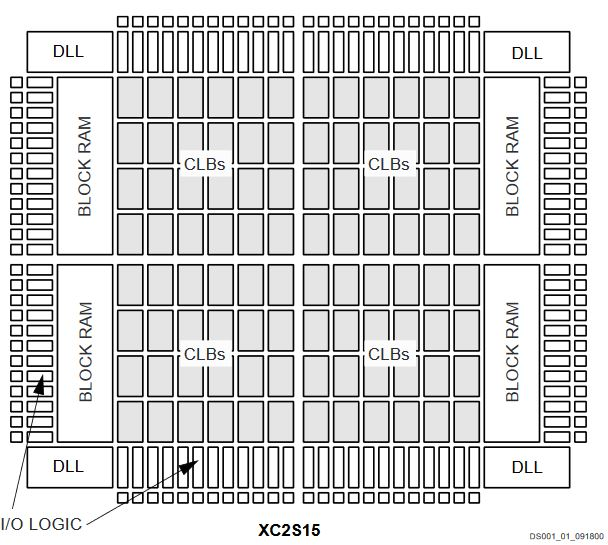
\includegraphics[scale=0.4]{fpga}
\end{center}
\caption{Xilinx Spartan-II FPGA layout \cite{spartan2}.}
\label{fig:}
%\end{wrapfigure}
\end{figure}

A field-programmable gate array (FPGA) is a reprogrammable logic device that enables digital electronic designs to be realised and executed on-chip. FPGAs utilise configurable logic blocks (CLB) that can be configured to emulate primitive gates. Connecting these primitive gates with others allows the engineer to realise complex logic such as combinational gates, multiplexers, and lookup-tables. Modern FPGA devices also include components such as block-RAMs, DLLs, and DSP blocks.

The embedded processor will be designed using the Verilog hardware description language (HDL). A HDL can be thought of as a front-end to a software compiler. Other HDL front-ends exist such as VHDL. The HDL is synthesised into an retargetable intermediate form consisting of nets - a form describing the gates, flip-flops, and their interconnections. After this synthesis takes place, the intermediate net list form is transformed into implementation specific forms. As this processor is designed for FGPA implementation, processes such as "place and route" are utilised to map the net list to physical resources on the FPGA. Different processes are performed for difference implementations, such as for ASICs and CPLDs.

\newpage
\chapter{Embedded Processors and Compilers}
{\hypersetup{linkcolor=black}
\startcontents[chapters]
\printcontents[chapters]{}{1}{}
}

\section{Introduction}
Modern computing and electronics equipment, like function generators, oscilloscopes, and spectrum analysers, use FPGAs to implement their compute intensive logic. These FPGAs are often accompanied by a small, low-cost, microprocessor to supervise and provide interfaces to external peripherals.

The aim of this project is to implement this side-microprocessor into the FPGA to save on BOM costs, PCB  space,  and  power  costs,  which  contribute  to  higher  development  and  product  costs.  While  savings can  be  made  by  the  lack  of  side  microprocessor,  the  product  may  need  a  larger  FPGA  to  accommodate the embedded microprocessor.  The project will produce a small, soft-core, CPU design and compiler. Although there is no direct client in this project, I believe this project will produce an attractive product
for FPGA-based product designers wishing to employ an embedded processor solution.

This report details the design considerations, implementation, and verification, of a new embedded processor architecture and a high-level code-compiler targeting it.

\section{Background}
Embedded processors are becoming more and more present in many products, ranging from toys to outdoor recording systems to test and measurement tools. In addition, FPGA-devices are being utilised in an increasing number of new areas, such as machine vision for image processing and machine learning.
 
\subsection{Soft-core Embedded Processors}
There exists many commercial and open-source embedded processors, each providing different features and specialities such as digital signal processing, analogue components, instruction set architectures, and interfaces.

Research has been performed to identify existing embedded processor features and characteristics. This research has been used to identify requirements and desired functionality of this new processor architecture. This research can be found in section \ref{current_impl} {\nameref{current_impl}}.


\newpage

\section{Project Overview}
This primary aim of this project is to improve my knowledge and experience in embedded processors, SoC design, computer architecture, and compilers. To do this, I will design an efficient and cost-saving alternative for board and hardware product designers utilising side-microprocessors by designing, implementing, and demonstrating, a small, portable, FPGA processor core design to be used in-place of the side-microprocessor. 

The processor core will implement it's own pipeline and instruction set architecture and so a compiler and assembler will also be provided so that software code can easily be executed on the processor. The new processor core and compiler tool chain will be named \textit{\scname{}}.

\subsection{Core Deliverables}
These core (C) deliverables are the base requirement for the project to be released in a functional and worthwhile state.
\begin{enumerate}[label=\bfseries C\arabic*.]
\item{To improve my knowledge and experience of FPGA development, processor architecture, compilers, and embedded systems engineering.}
\label{c1}
\item{To build a working and operational soft-core processor core capable of performing simple tasks.}
\item{Implementation of the soft-core processor design on real hardware (FPGA).}
\item{To provide a high-level context-free code compiler to run user-code on the processor.}
\end{enumerate}

\subsection{Extended Deliverables}
These extended (E) deliverables may not be achievable in the time frame specific in section \ref{sect:proj_time} as they may require extra time to design and implement, require more experience or skill, or require resources currently unattainable.
\begin{enumerate}[label=\bfseries E\arabic*.]
\item{To provide a technical processor reference guide and specification for the embedded core.}
\item{To provide embedded products a convenient solution to in-field updating.}
\item{To provide product designers with an affordable alternative to a side-microprocessor in their FPGA-based products.}
\item{To provide easy interfacing between the FPGA design and the embedded core.}
\item{GCC/LLVM/8CC compiler backend for C programming.}\label{sect:deliv:ed:gcc}
\item{Wishbone interface for easier modularity and inter-module communication.}
\item{Multi-core design with Wishbone (2).}
\item{Configurable build options (register/bus widths, optimisations/pipelining, user/privileged mode to support modern operating systems).}
\item{Memory management modules to provide protected and virtual memory lookup tables.}
\end{enumerate}


\section{Legal and Ethical Considerations}
This project adheres with the University of Plymouth's Ethics Policy \cite{ethics}.

\subsection{Privacy}
The \scname{} processor will be able to read and write to all data passing through it and control all connected peripherals (such as UARTs, SDRAMs, and SD Cards). The processor does not track or store usage behaviour, instructions and their frequency,   memory contents, or timing statistics, or any other usage metric.

\subsection{Fit for Purpose}
The \scname{} processor is \textbf{not} designed to run general purpose operating systems, such as Linux or embedded RTOS systems. All memory devices attached to the FPGA are fully accessible to the processor core and instructions/programs running through it, meaning that operating systems or secure applications storing private and sensitive information is not protected by modern processor features such as privilege modes and virtual memory sections. The processor lacks common components required to run modern operating systems, such as a memory management unit (MMU) and privilege modes, and so \textbf{should not be run on the processor}.

The \scname{} processor is \textbf{not} designed to run in high-reliability or safety-critical environments that require established safety standards, such as the UK Defence Standard 00-56 \cite{defstan_0056_2} and IEC 61508 \cite{iec61508}.

The \scname{} processor is \textbf{not} designed for implementation in silicon and makes no guarantees of reliability or performance in this format. The \scname{} processor, by design, should be used as a replacement for a simple micro-controller accompanying a main processing module.

\subsection{Third-party Libraries}
This project uses only 1 external library for the processor core's universal asynchronous receiver-transmitter (UART) module that does not depend on any other libraries. This allows me to guarantee that: the project rights are secure; and application behaviour is well-defined and predictable (no exploits introduced/injected from external libraries). The UART module does feature a large first-in-first-out (FIFO) buffer for temporary storage of in- and out- going messages. This FIFO is internal to the FPGA design and so is protected from external viewing/modification by probing the board in which the core is running on.

The compiler sub-project does not use any external library dependencies, does not record telemetry or usage statistics, and does not require an internet connection to run.

\subsection{Generated Code}
The \scname{} compiler will not insert telemetry or any other kind of usage tracking into the generated code.
The code generated by the compiler is \textbf{not guaranteed} to:
\begin{itemize}
\item{\textbf{Produce code for secure environments}. The compiler will not randomise, obfuscate, or split-up and spread, output code. Output machine code will be in a predictable format (global variables in low-memory, instruction memory in middle-memory, and stack memory in high-memory) making the binary easily subject to reverse-engineering and modification.}
\item{\textbf{Produce constant time executable code for expressions}. For example, the compiler output for an \textit{if} statement may implicitly vary depending on it's condition expression, which may have been optimised out, constant-folded, or without-optimisation. This also applies for user code aiming to create reliable and accurate time delay loops; although the processor does not perform optimisations such as instruction caching or branch prediction, access to memory and ALU operations may vary in time, resulting in unreliable instruction times.}
\end{itemize}



\chapter{Project Management}
{\hypersetup{linkcolor=black}
\startcontents[chapters]
\printcontents[chapters]{}{1}{}
}

\section{Method of Approach}
Development of the \textbf{core} and \textbf{compiler} will be done in separate stages of the project (see section \ref{sect:proj_time}). The two deliverables will be split into 2 sub-projects. Both sub-projects will employ the \textbf{Agile development process}, using Agile's sprints to split up tasks into sub-tasks and Agile's scrums to discuss progress, features, and changes. This technique allows revisiting of tasks to tweak and iterate over their implementation which will be key when for incrementally adding features to both sub-projects, for example, adding to the core's ALU module to add conditional branching, or adding new instructions to the core's decoder module if required.

This project will be split into 4 main stages: First is the requirements and information gathering as well as finalising core and compiler features (such as registers and instructions). The second stage consists of the design, implementation, and verification  of the embedded processor core. The third stage consists of the implementation of the compiler and verification for it. The final stage is dedicated to reviewing the project and the final report. This is further described in section \ref{stages}.

This project combines the benefits of Agile and PRINCE2 methodologies. In particular, we align highlight reports with the projects stages and work on each stage in sprints. The contents and review of each sprint can be found in the highlight reports.

In addition, a Kanban board is used to track current sprint challenges, such as bugs and feature implementation statuses. Figure \ref{kanban} shows the project's Kanban board with tasks for open bugs and features.



\section{Resources and Dependencies}
For the first half of the development cycle, the core can be developed and verified using the Verilog simulator and test suite, \textbf{Verilator}, and VHDL and Verilog simulator, \textbf{iSim}.

The second half of development will require deploying and debugging on real hardware. This will require an FPGA development kit. To better emulate customer products, the development kit should feature common components such as LEDs, GPIO, USB interface, flash-based storage and memory, and optionally an analogue audio output port. The low-middle range of FPGA devices the project is targeting is the popular and affordable yet feature rich Spartan-6 and Artix-7 FPGAs. From my placement, I have gained experience in Xilinx FPGAs and so will be targeting them for this project to reduce risk and development time.
\\\\
The following FPGA development kits are suitable for this project:
\begin{enumerate}
\item{MiniSpartan6+ - Scarab Hardware - £79 (already owned) \cite{scarabhardware}. The MiniSpartan6+ features a Spartan-6 XC6SLX9 FPGA, 8 LEDs, 2 digital and analogue headers, FT2232 FTDI USB to JTAG, 64Mb SPI flash memory, 32MB SDRAM, an audio output jack, and a MicroSD socket.

\begin{figure}[H]
\centering
     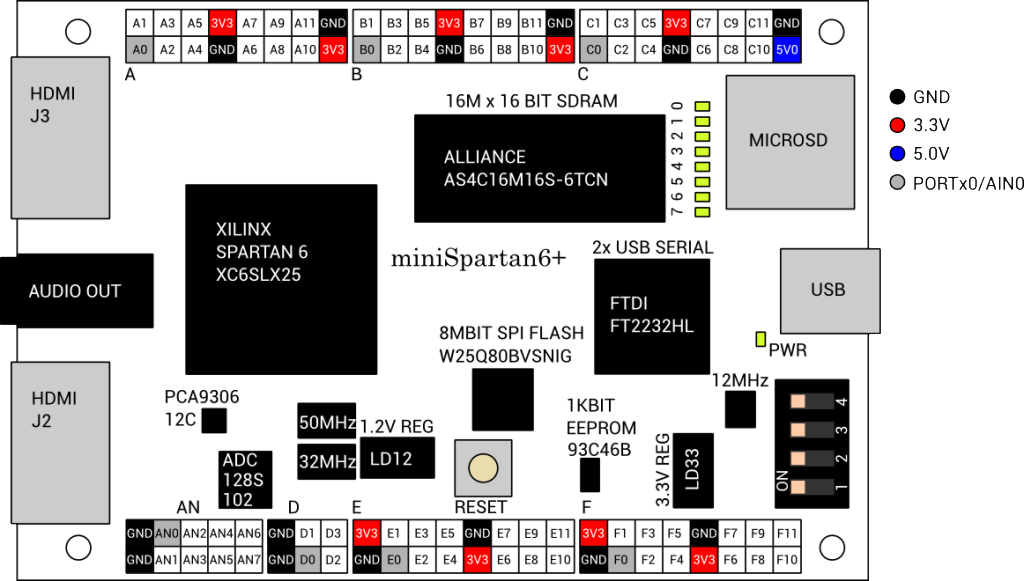
\includegraphics[width=0.5\textwidth]{minispartan}
      \caption{Scarab Hardware MiniSpartan6+ board layout.}
       \label{fig:res:minispartan}
\end{figure}
}
\label{res:minispartan}

\item{Arty Artix-7 FPGA Development Board - Digilent - £100 \cite{arty}. The Arty development board features a larger Artix-35T FPGA with over 20x the number of logic cells and block memory compared to the LX9 in the MiniSpartan6+. The board components include 256MB DDR3 RAM, 16MBx4 SPI flash memory, USB-JTAG, 8 LEDs (4 of which are RGB), 4 switches, 4 buttons, and multiple Pmod connectors.
\\\\
The greater number of IO options and larger FPGA make the Arty board better suited to emulating real customer products.


\begin{figure}[H]
\centering
     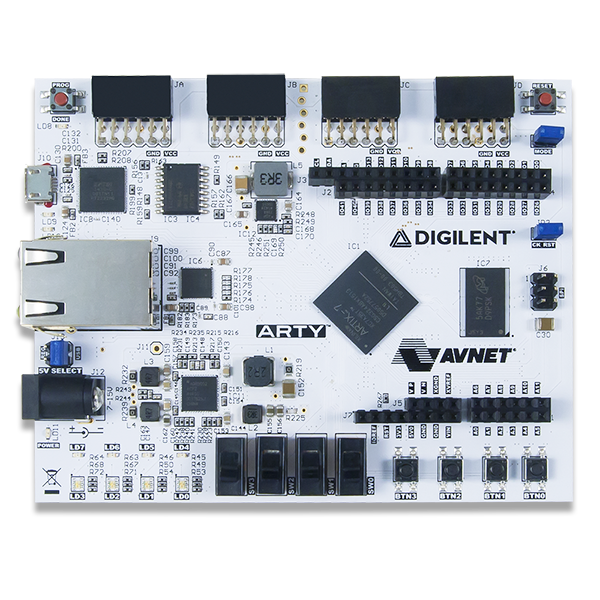
\includegraphics[width=0.5\textwidth]{arty}
      \caption{Digilent Arty Artix-7 board.}
       \label{fig:res:arty}
\end{figure}
}
\end{enumerate}

Although the Arty Artix-7 FPGA development board was identified as the most beneficial development board for this project, it was decided to use the MiniSpartan-6+ development board due to my existing familiarity with the Spartan-6 FPGA family and tools. If the Artix-7 FPGA was used, additional time and resources would need to be allocated to learning and getting the Vivado software suite set up.

The project will require a computer or laptop to develop the core and compiler on and continuous integration systems to perform testing on the incremental builds. For the project demo, an oscilloscope (already owned) or digital logic analyser may be required to demonstrate some of the core's features.

\subsection{Source Control}
Version control will be utilised to improve work-flow, reference and review code changes, and protect the project from data loss and corruption. GitHub, a git hosting provider, will be utilised to host all project files, including documentation and design files.

The repository can be found here: \href{https://github.com/bendl/prco304}{https://github.com/bendl/prco304}

\begin{figure}[H]
\centering
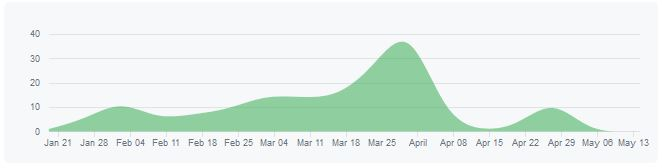
\includegraphics[scale=0.7]{github}
\caption{Chart showing the frequency of commits over the life cycle of the project.}
\end{figure}

\subsection{Document Control}
All documents will be authored in LaTeX and markdown. This allows all documents to follow a custom style guide, share resources, and display complex visualisations (such as syntax highlighting), and has great support for version control and collaboration.

All documentation is stored in the \verb|prco304| GitHub repository (URL above) in the \verb|doc/| directory alongside the source directories (\verb|prco_compiler/| and \verb|prco_core/|). By including documentation with sources, a pattern employed by large open-source projects such as GCC, Linux, and CPython, allows future projects utilising the resources in this project to easily navigate, understand, and contribute back to the project.

\section{Stages}
\label{stages}
\label{sect:proj_time}
The project is organised into 4 distinct stages: 1. Research, requirement gathering, and initial design; 2. Processor core implementation; 3. Compiler implementation; and 4. Project conclusion.

\begin{figure}[H]
\centering
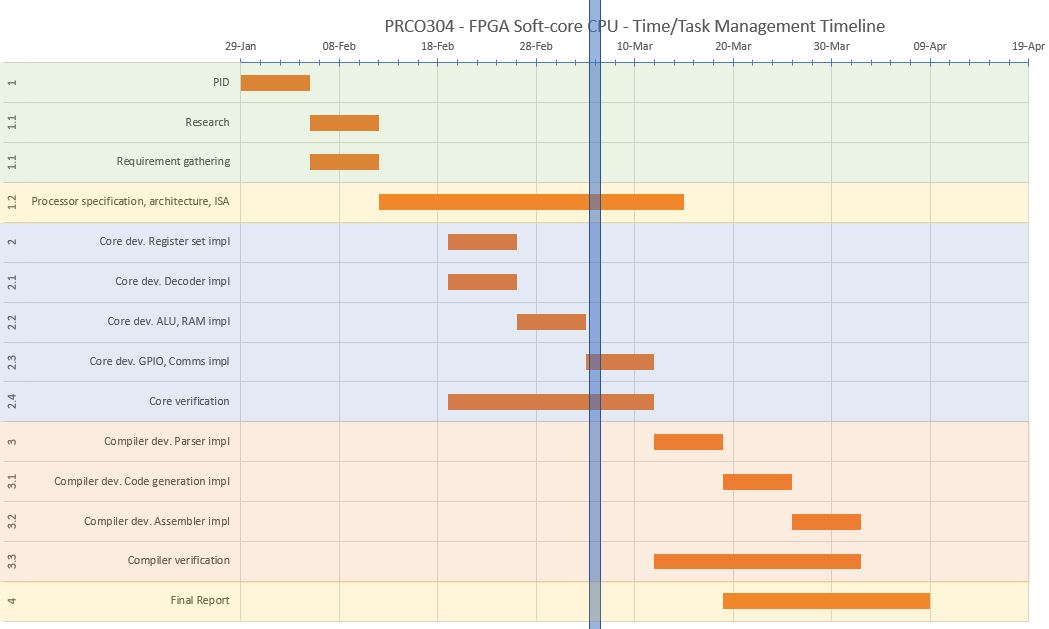
\includegraphics[scale=0.6]{gantt}
\caption{The project's gantt time chart showing project stages, times, and deadlines. The vertical blue bar shows the current time of the project.}
\label{fig:proj_time}
\end{figure}

\subsection*{Stage 1.0: Project Initiation Document}
A PRINCE2 Project Initiation Document (PID) is provided in {\nameref{pid}}. This documentation is used to initial propose the project to managing personnel by listing project requirements, objectives, risks, and quality plans.

\subsubsection*{Stage 1.1: Research and Requirement Gathering}
This stage is used to research existing embedded processors and compilers. This information is used to aid creating SMART (Specific, Measurable, Achievable, Relevant, Timely) project objectives and deliverables.

\subsubsection*{Stage 1.2: Core \& Compiler high level design}
This stage covers the high level design of the processor core. A specification is written up to describe components of the processor core, such as register sets, instructions, pipe-lining, and control systems.

The compiler high-level design specifically covers program flow, internal structures for representing the input code, and software paradigms that will be employed.

As seen in Figure \ref{fig:proj_time}, this task is allocated over 1 month of time. This is because Agile methodologies will be employed. Frequent reviews will held at the end of each highlight report. These reviews may suggest that new instructions or timing changes are required, and so the high-level design will be continuously updated.
\\\\
Stages 2.0 and 3.0 are described in more detail in their own chapters (Chapter \ref{core}, Chapter \ref{compiler}). 

\subsection*{Stage 2.0: Core Register-set Implementation.}
Once the core high level design in complete, implementation of the register set is started. This is a key component of the core as it is connected to multiple other components, such as the decoder and ALU.

\subsubsection*{Stage 2.1: Core: Decoder Implementation.}
The decoder is used to identify operands within machine code instructions. The decoder is a simple and fast component; The current instruction is it's input, and it outputs the instructions operands, such as register selectors and immediate values. It is connected to the RAM and register components, to fetch instructions and get register contents respectively.

\subsubsection*{Stage 2.2: Core: ALU, RAM Implementation.}
This stage is used for implementation of the Arithmetic Logic Unit (ALU) and Random-access Memory (RAM). The ALU is used for performing arithmetic, logical, and address functions on data coming from the register set. The ALU result is then either piped back to the register set or sent to the RAM module for mass storage.

\subsubsection*{Stage 2.3: Core: GPIO, Communication.}
This stage implements external user interfaces that allow the processor core to read and write data and messages to other devices outside the core. Specifically, implementation for a UART transmitter and a debugging instruction-stepper button are performed.

\subsubsection*{Stage 2.4: Core: Verification.}
This stage is used to meet quality requirements stated in the ({\nameref{pid}}. To meet these quality requirements, multiple forms of verification and testing is performed, such as manual simulation of the core design and automatic unit tests. This stage is continuously performed throughout the development of the processor.

\subsection*{Stage 3.0: Compiler:. Parser impl.}
This stage starts the implementation of the compiler's front-end. The compiler must be able to read an input file character by character and to create an internal representation of this data.

\subsubsection*{Stage 3.1: Compiler: Code-generation.}
This stage implements the compilers output code-generator. Given an Abstract Syntax Tree (AST), the compiler will decide on and run code-generation routines to emit machine-code instructions for use by the processor core.

\subsubsection*{Stage 3.2: Compiler: Assembler.}
The assembler takes an initial list of machine code instructions and calculations missing information that could not be calculated before, such as addresses and offsets. After the assembler has ran, the output machine code should be in an executable state.

\subsubsection*{Stage 3.3: Compiler verification}
Like Stage 2.4, this stage is present throughout the development life-cycle of the compiler. Automatic unit tests and continuous integration tests are performed on the compiler for every code change to verify correct operation of the compiler. This achieves the projects quality requirements.

\subsection*{Stage 4.0: Report.}
The final stage is dedicated to the post-project tasks. This involves reviewing original project objectives and deliverables, ensuring all risks have been resolved, and writing of the final report. 



\chapter{\scname{} Processor Design}
\label{core}
{\hypersetup{linkcolor=black}
\startcontents[chapters]
\printcontents[chapters]{}{1}{}
}


\section{Introduction}
The \scname{} Processor Design is the first of two deliverable sub-projects required for this project. The processor is designed to be a small, instantiated, Verilog module that can be easily inserted into existing FPGA-based Verilog projects.



\newpage
\section{Project Management}
Using research gathered from existing embedded processor designs (see section \ref{current_impl}), and consideration of constraints such as time and resources (see section \ref{sect:proj_time}), the following core and extended deliverables have been decided:

\subsection{Core Deliverables}
The following Core Processor Deliverables (CPD) are deliverables that must be implemented for the processor to be deemed functional. These goals were designed with SMART methodologies in mind.

\begin{enumerate}[label=\bfseries CPD\arabic*.]
\item{Support a wide range of executable programs.}
\item{Provide a 16-bit instruction set capable of supporting simple programs (recursion, memory reading, strings (arrays), function calling).}
\item{Support simple arithmetic and bitwise operations (ADD, SUB, OR, XOR, etc.).}
\item{Operate on 16-bit data sizes (16-bit register and instruction sizes).}
\item{Fully synthesize-able on FPGA hardware.}
\item{Implement a simple pipeline architecture.}
\end{enumerate}

\subsection{Extended Deliverables}
The following Extended Processor Deliverables (EPD) are deliverables that must be implemented for the processor to be deemed functional.
\begin{enumerate}[label=\bfseries EPD\arabic*.]
\item{Provide hardware-based multiplication, division, modulus, instructions.}
\item{Provide SIMD style instructions for faster vector manipulation.}
\item{Provide in/out GPIO and UART modules for external communication.}
\item{Provide an interrupt system allowing asynchronous events to be handled.}
\item{Implement a super-scalar pipeline architecture (execute more than 1 instruction per clock).}
\end{enumerate}

\subsection{Applicable Stages}
The design, implementation, and verification of the new processor consist of the  project stages 1.2 to 2.4. Initially described above in section \ref{stages}, below details additional technical considerations, challenges, and changes that occurred during these stages.

\begin{description}[style=nextline]
\item [Stage 1.2: Processor specification, architecture, ISA]
As discussed in section \ref{current_impl}, existing embedded processors have been researched and compared in order to determine a suitable and realistic specification for the processor  design. A comparison table is also available in appendix \ref{sect:existing_isa_cmp}.


\item [Stage 2.0: Core dev. Register set implementation]
This stage covers the implementation of the register set in Verilog, as per the specification. 
After this stage, the processor will be able to read and write 16-bit values in the dual port register set.

\item [Stage 2.1: Core dev. Decoder implementation]
The instruction decoder is a core part of all processors; they deconstruct incoming instructions and identify operands within the instruction, such as immediate values, opcodes, and register selects. The decoder went through an iterative development utilising Agile sprints. This allowed new instructions to be iteratively added to the module to support new features.



\item [Stage 2.2: Core dev. ALU, RAM implementation]
Like the decoder, the ALU was required to implement changing instruction definitions, such as status register bits and comparison operands. Initially, the status register was included in the register set as a dedicated register, but it was later changed to a local register accessible only to the ALU. This was because the register set 

\item [Stage 2.3: Core dev. GPIO, Comms implementation]
UART and GPIO interfaces are implemented in the processor. These can be accessed by using the \verb|READ| and \verb|WRITE| instructions.

\item [Stage 2.4: Core verification]
To ensure quality requirements (\ref{quality}) are achieved, multiple verification and testing strategies were employed, such as simulation, unit testing, and emulation. These are described in further detail in section \ref{sect:core_test}.
\end{description}


\newpage
\section{High Level Design}
The \scname{} processor is a modularised processor with independent components for the ALU, Registers, RAM, and it's peripherals.  Figure \ref{fig:core_hld} below shows how the processor core can be integrated onto the MiniSpartan-6+ development kit and connected to peripherals.

\begin{figure}[H]
\begin{center}
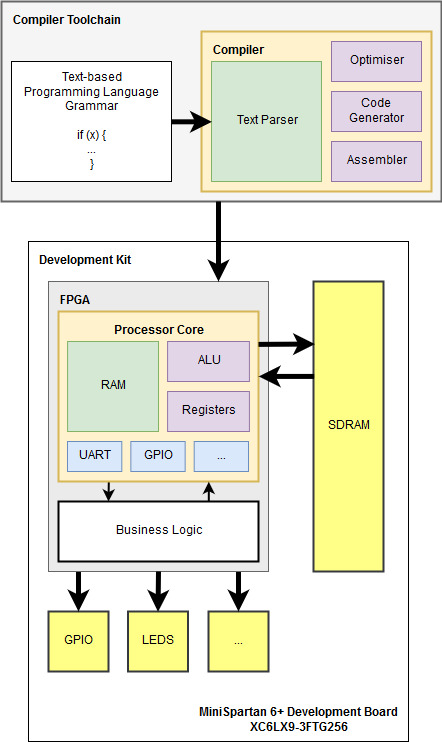
\includegraphics[scale=0.5]{hld}
\end{center}
\caption{\scname{} processor block diagram showing component interconnections within the processor, FPGA, and development board.}
\label{fig:core_hld}
\end{figure}

\section{Registers}
\scname{} has a total of 8 addressable, read and write, registers. These registers are identified by letters A through H.

\subsection{General Purpose Registers}
Registers A through E are designed for general purpose use and are safe to store user values over the run-time of the processor.

\begin{table}[h]
\def\arraystretch{1.3}%  1 is the default, change whatever you need
    \begin{tabularx}{\textwidth}{|p{2cm}|l|X|}
    \hline
    Registers & Bits & Description \\
	\specialrule{2pt}{-2pt}{0pt}
	A through E & 15:0 & 5 General purpose registers
	\\ \hline
    \end{tabularx}
    \caption{General purpose registers.}
\end{table}

Instructions that require a destination register, such as CMP, can reference any register (even special registers if that is your requirement). For the CMP instruction as an example, the processor will put the result of the comparison instruction in the destination register, overwriting any value present in that register.

\subsection{Special Registers}
Registers F through H are special registers within the processor. The processor cannot guarantee that a value written or read in these registers will persist over the run-time of the processor. Erroneously writing to these registers may severely affect program and processor behaviour.

Even though all registers can be used at the will of the programmer, it is recommended to isolate a few registers to provide special features, such as RAM stack management, interrupts, and IO multiplexing.

\begin{table}[h]
\def\arraystretch{1.3}
    \begin{tabularx}{\textwidth}{|p{2cm}|l|X|}
    \hline
    Registers & Bits & Description \\
	\specialrule{2pt}{-2pt}{0pt}
	F & 15:0 & {\nameref{sect:core_regs_sr}}
	\\ \hline
	G & 15:0 & {\nameref{sect:core_regs_bp}}
	\\ \hline
	H & 15:0 & {\nameref{sect:core_regs_sp}}
	\\ \hline
    \end{tabularx}
    \caption{Special registers.}
\end{table}

\subsubsection{Status Register}
\label{sect:core_regs_sr}
The Status Register is a dedicated register used by the ALU to provide additional information on results of instructions. Using the Status Register is essential for programs wanting to perform conditional branching or operate on dynamic data.

\begin{table}[h]
\def\arraystretch{1.3}
    \begin{tabularx}{\textwidth}{|p{2cm}|l|X|}
    \hline
    Bit & Name & Description \\
	\specialrule{2pt}{-2pt}{0pt}
	0 & SR\_Z & Set if the result of a CMP instruction is 0.
	\\ \hline
	1 & SR\_S & Set if the result of a CMP instruction is signed (greatest bit is 1) (signed).
	\\ \hline
	2 & SR\_O & Set if the result's 17'bit of a CMP instruction's is set (overflowed).
	\\ \hline
    \end{tabularx}
    \caption{Status Register breakdown.}
\end{table}

These bits are chosen as they can be combined to represent different types of comparison, such as \textit{equal to}, \textit{greater than}, and \textit{less than or equal to}. 

\subsubsection{Base Pointer}
\label{sect:core_regs_bp}
The \scname{} processor assumes that the compiler will employ a stack management scheme similar to that of x86 machines. By doing so, the compiler assumes the last 2 registers are dedicated to stack management. The Base Pointer register is used in a similar way to the x86 Base Pointer register.

Compilers and code generators should utilise this register for storing the address of the current stack frame. By utilising the register this way, features such as local and passed variables become available as they are addressable by offsetting the Base Pointer by a constant value.

\subsubsection{Stack Pointer}
\label{sect:core_regs_sp}
The Stack Pointer is similar to the x86 Stack Pointer in that it stores the address of the top of the stack. This register is used primarily for PUSH and POP operations (see section \ref{sect:compiler_cg_push_pop} {\nameref{sect:compiler_cg_push_pop}} for example usage).

\section{Instruction Set Architecture}
\label{sect:isa}
The chief project objective, \ref{c1}, is to improve my knowledge of FPGA development, processor architecture, and embedded systems. To do this, it was decided with the project supervisor to design and implement a new instruction set architecture (ISA) aimed specifically for this embedded processor. In addition to improving my knowledge and experience, it would avoid legal and ethical issues introduced if emulating an existing architecture, such as MIPS, ARM's Thumb2, or x86.

The use of Agile development was beneficial in the design of the ISA. As the processor  was developed and programs were ran on the processor, the need for new instructions and requirements were observed. For example, it was observed that code generation for boolean comparisons (e.g. \verb|a < b|) could be reduced by introducing a new instruction, \verb|SETC|, therefore increasing program speed, reducing file size, and improving debugging. This is described further in section SETC \ref{setc}.
\\\\
The \scname{} processor implements it's own fixed 16-bit little-endian instruction set. A 5-bit opcode is present in each instruction, identifying the type of instruction. This allows for $2^5$ (32) unique instructions. However, this can be extended if unused bits in instructions are utilised. 


\subsection{Instruction Types}
It was decided to support the following 3 types of instructions. This allows for a wide range of instruction operands, such as more registers selectors or larger immediate values.

\begin{table}[h]
\def\arraystretch{1.3}
\centering
\begin{tabular}{|p{4cm}|c|c|c|c|}
\hline 
Type & \multicolumn{4}{c|}{Bits} \\ 
\specialrule{2pt}{-2pt}{0pt}
\hline 
Type 1 & 15-11 & 10-8 & 7-5 & 4-0 \\ 
\hline 
Type 2 & 15-11 & 10-8 & \multicolumn{2}{c|}{7-0} \\ 
\hline 
Type 3 & 15-11 & \multicolumn{3}{c|}{10-0} \\ 
\hline 
\end{tabular}
\caption{The 3 instruction format types used by the \scname{} processor.}
\end{table}

\subsection{Instructions}
\begin{table}[H]
	\def\arraystretch{1.3}
    \begin{tabularx}{\textwidth}{|p{4cm}|c|c|c|c|X|}
    \hline
    Type 1 & 15-11 & 10-8 & 7-5 & 4-0 & Semantics\\ 
	\hline 
	Type 2 & 15-11 & 10-8 & \multicolumn{2}{c|}{7-0} & Semantics \\ 
	\hline 
	Type 3 & 15-11 & \multicolumn{3}{c|}{7-0} & Semantics\\ 
    \specialrule{2pt}{-2pt}{0pt}
    
    NOP 	& 00000 & X & X & X & PC $<$= PC + 1 \\ \hline
    LW 		& 00001 & Rd & Ra & Simm5 & Rd $<$= RAM[Ra + Simm5] \\ \hline
    SW 		& 00010 & Rd & Ra & Simm5 & RAM[Ra + Simm5] $<$= Rd \\ \hline
    MOV		& 00011 & Rd & Ra & X & Rd $<$= Ra \\ \hline
    MOVI 	& 00100 & Rd & \multicolumn{2}{c|}{Simm8}  & Rd $<$= Simm8 \\ \hline
    ADD 	& 01000 & Rd & Ra & X & Rd $<$= Rd + Ra \\ \hline
    ADDI 	& 01001 & Rd & \multicolumn{2}{c|}{Simm8}  & Rd $<$= Rd + Simm8 \\ \hline
    SUB		& 01010 & Rd & Ra & X & Rd $<$= Rd - Ra \\ \hline
    SUBI 	& 01011 & Rd & \multicolumn{2}{c|}{Simm8}  & Rd $<$= Rd - Simm8 \\ \hline
    JMP		& 01100 & Rd & \multicolumn{2}{c|}{Imm8} & See {\nameref{sect:isa_jmp}}. \\ \hline
    CMP		& 01101 & Rd & Ra & X & Set SR flags \\ \hline
    HALT	& 10010 & \multicolumn{3}{c|}{X} & Stop the processor. \\ \hline
    WRITE	& 10011 & Rd & \multicolumn{2}{c|}{Imm8} & PORT[Imm8] $<$= Rd \\ \hline
    READ	& 10100 & Rd & \multicolumn{2}{c|}{Imm8} & Rd $<$= PORT[Imm8] \\ \hline
    SETC	& 10101 & Rd & \multicolumn{2}{c|}{Imm8} & Set Rd to 1 if Imm8 is set in {\nameref{sect:core_regs_sr}} from last CMP instruction, else 0. \\ \hline
    \end{tabularx}
    \caption{All \scname{} processor instructions and their semantics. Detailed descriptions of each instruction is provided in {\nameref{appendix:isa}}.}
\end{table}

\subsection{Conditional Branching}
\label{sect:isa_jmp}
Table \ref{tab:isa_jmp_bits} below details each conditional branch parameter and how it is evaluated in the {\nameref{sect:core_regs_sr}}.

\begin{table}[H]
	\centering
	\def\arraystretch{1.5}
    \begin{tabularx}{\textwidth}{|c|c|c|c|c|X|X|}
    \hline
    & 15-11 & 10-8 & \multicolumn{2}{c|}{7-0} & Semantics & {\nameref{sect:core_regs_sr}} \\
    \specialrule{2pt}{-2pt}{0pt}
    JMP		& 01100 & Rd & \multicolumn{2}{c|}{0000 0000} & Unconditional Jump & Any\\ \hline
    JE		& 01100 & Rd & \multicolumn{2}{c|}{0000 0001} & Jump Equal & SR\_Z=1\\ \hline
    JNE		& 01100 & Rd & \multicolumn{2}{c|}{0000 0010} & Jump Not Equal & SR\_Z=0\\ \hline
    JG	& 01100 & Rd & \multicolumn{2}{c|}{0000 0011} & Jump Greater Than & SR\_Z=0 and SR\_S = SR\_O\\ \hline
    JGE		& 01100 & Rd & \multicolumn{2}{c|}{0000 0100} & Jump Greater Than or Equal & SR\_S = SR\_O\\ \hline
    JL		& 01100 & Rd & \multicolumn{2}{c|}{0000 0101} & Jump Less Than & SR\_S$<>$SR\_O\\ \hline
    JLE		& 01100 & Rd & \multicolumn{2}{c|}{0000 0110} & Jump Less Than or Equal & SR\_Z=1 or SR\_S$<>$SR\_O\\ \hline
    JS		& 01100 & Rd & \multicolumn{2}{c|}{0000 0111} & Jump Signed & SR\_S=1\\ \hline
    JNS		& 01100 & Rd & \multicolumn{2}{c|}{0000 1000} & Jump Not Signed & SR\_S=0 \\ \hline
    \end{tabularx}
    \caption{Conditional jump instructions showing how the Status Register is utilised.}
    \label{tab:isa_jmp_bits}
\end{table}

\subsection{Design Considerations}
As stated in section \ref{sect:isa} above, the use of agile methodologies allowed for constant review of the functionality of the processor. After these reviews, design changes were proposed, tested, and integrated into the processor.

The \scname{} processor's ISA has been through multiple iterations; from opcode length changes, operand bit position changes, and immediate value sizes. The following sections describe some of the design considerations and changes of the \scname{} processor.

\subsubsection*{Opcode Bits} 
Initially, the opcode length was 4-bits allowing a total of 16 unique opcodes. This was later changed to 5-bits to add more opcodes at the cost of addressing fewer registers and having smaller immediate values. This change was enabled by using the agile methodology.

\subsubsection*{Multiplication and Division}
Due to time constraints, multiplication or division instructions are not implemented within the \scname{} processor. The equivalent functionality and more can still be achieved using the currently available instructions. The test file \verb|prco_compiler/test/tests/mul_1.prco| and \verb|prco_compiler/test/tests/div_1.prco| contain example unsigned integer multiply and divide functions.

\subsubsection*{SETC Instruction}
\label{setc}
The \verb|SETC| instruction was added to reduce the number of instruction required to perform boolean logic operations on registers. Without the \verb|SETC| instruction, to evaluate the expression \mintinline{c}{1 < 5}, the compiler would need to emit multiple JMP instructions to set the result to 0 or 1 and JMP over the other result. In my testing, the compiler would require between 5-8 instruction for each boolean expression. 

The \verb|SETC| instruction is inspired by the x86 instruction: \verb|SETcc| Set Byte on Condition \cite{isa_x86}.

With the introduction of the \verb|SETC| instruction late in development, the number of instructions could be reduced to around two instruction. (one for the initial comparison, and one for setting 1 or 0 with \verb|SETC|). This greatly improved program execution time and size.


\section{Pipeline Architecture}
\label{core:pipeline}
The \scname{} processor employs a \textit{feed-forward} pipeline strategy. 
This pipeline supports:
\begin{itemize}
\item{Time-varying processes: Multi-clock cycle decoding; Memory access; ALU operations.}
\item{Module re-ordering: Instruction dependencies; Module skipping; Output redirection.}
\end{itemize}

As the pipeline is feed-forward, no information is sent back to previous modules to tell them of their status. This means that if a module is stalled (due to mutli-cycle processes or future modules are stalled), and the previous module is ready, the previous module will signal the next module that information is ready and it should take it, but the current module is unable to as it is busy. The pipeline resolves this issue by it's cyclic nature. This means that only 1 module at any time is processing data. Of-course, the downside to this approach is that instruction parallelism is reduced.

\begin{figure}[ht]
\centering
     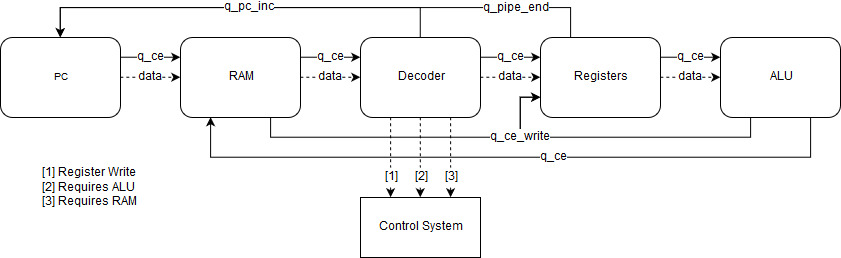
\includegraphics[width=1.0\textwidth]{prco_forward_pipe}
      \caption{The feed-forward pipeline interconnect diagram used by the \scname{} processor.}
       \label{fig:prco_forward_pipe}
\end{figure}

The pipeline structure is described in figure \ref{fig:prco_forward_pipe} (above). The general order of the modules is shown from left to right, but this can change due to the pipelines re-ordering functionality.

The Decoder module will decode instruction words from memory and will output appropriate signals containing the requirements of the instruction, such as requiring register write access, any ALU operation, and whether the instructions requires access to internal/external memory.
\newline\newline
To improve instruction performance, the decoder can also choose what modules are required and when they are called. For example, for the {\nameref{isa_movi}} (move immediate) instruction the Decoder will assign the following modules in the following order: ALU and Register write, resulting in a total of 5 stages (including PC, Fetch, and Decode). The last module in this pipeline, the Register write, will raise the \textit{q\_pipe\_end} signal indicating that the pipeline has finished and to start fetching the next instruction.

For the NOP instruction, the decoder identifies that the instruction requires no dependencies and will hence raise the \textit{q\_pc\_inc} signal resulting in only 3 pipeline stages.

For instructions that require RAM access, a typical pipeline order might look like: PC, Fetch, Decoder, Register Read, ALU, RAM, resulting in 6 stages being used.

\begin{figure}[H]
\begin{center}
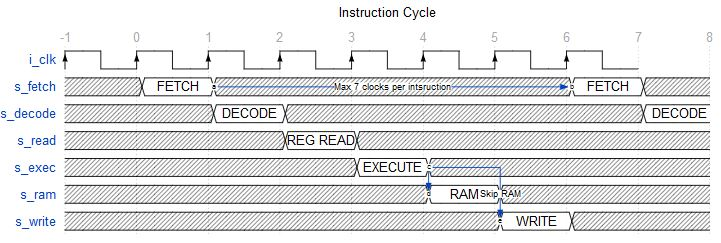
\includegraphics[scale=0.8]{td_instr}
\end{center}
\caption{\scname{} processor instruction cycle time diagram.}
\label{fig:dft_algorithm}
\end{figure}

\section{Testing and Verification}
\label{sect:core_test}
Multiple forms of verification and validation are performed on the processor to satisfy the quality requirements (\ref{quality}) of the project.

\begin{itemize}
\item{\textbf{Verilator testbenches} are used to automatically verify correct behaviour of the RTL code. These testbenches use the Verilator framework to compile and simulate Verilog modules. These tests produce an output report detailing test results and real register values. 
The Verilator test benches used in this project are found in \verb|prco_core/rtl/test/verilator| and can be run using the script: \verb|make_test.sh|.

\begin{minted}{text}
Running test: ALU OR 2
ALU_OP_WRITE/READ 000a
PASS: 10 10

Running test: ALU OR 3
ALU_OP_WRITE/READ 0004
FAIL: Got 4 Expected 7
=============================
14/27 tests passed.
\end{minted}
An example test report for the ALU running OR instructions on different operands and immediate values is shown above.
}

\item{\textbf{iSim testbenches} are used to better visualise signal states and changes over time. These testbenches require manual verification and so it can take a considerable amount of time to verify a module.

\begin{figure}[H]
\begin{center}
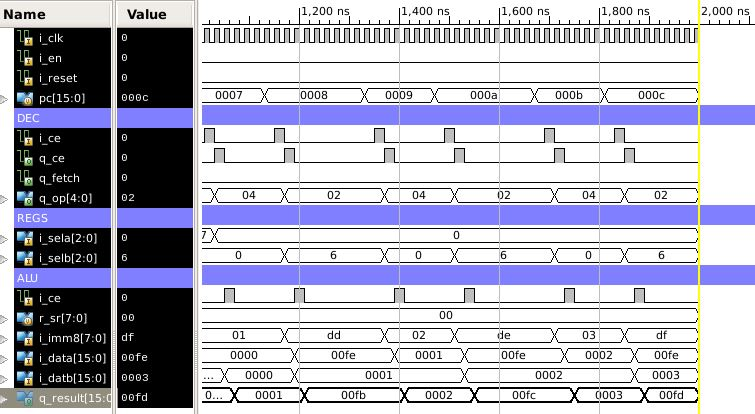
\includegraphics[scale=0.5]{core_test_isim}
\end{center}
\caption{iSim simulation showing high-level signals in the processor core, including: Program Counter (pc); current Op code (q\_op); and ALU result (q\_result).}
\label{fig:core_test_isim}
\end{figure}
}

\item{\textbf{Single-step implementation runs} are used to verify the correct behaviour of the RTL code on a real FPGA device. 

The \scname{} processor core features a single-step input line that can be pulsed to signal the core to execute the next instruction. In these tests, generally the first register Ax is redirected to the 8 LEDs on the development board, allowing the tester to visually see it's contents. However, only the higher-or-lower byte can be viewed at any single time (as registers are 16-bits wide). UART printing is also used to visualise register contents, however, integer to ASCII conversion is not implemented so only single digits can be displayed in ASCII.}
\end{itemize}



\newpage
\section{Core Analysis}
\label{sect:core_analysis}

\subsection{ISE Implementation Report}
\label{ise_impl}
In the ISE suite, reports are generated for synthesis, place-and-route, and programming file generation. These report detail how resources on the physical device are utilised in the HDL design, for example the number of slices, LUTs, latches, and block RAMs.

The full implementation report for the \scname{} processor is listed in \ref{ise_report} {\nameref{ise_report}}. An important characteristic is the number of slices the FPGA supports. The XC6SLX9 Spartan-6 FPGA used in this project has 1,430 slices available. From the implementation report, it can be seen that the \scname{} processor uses 844 (59\%) of the available slices. Although the Spartan-6 device used is a small FPGA, the number of slices used is still high, indicating inefficiencies in my HDL design.

It can be seen that the number of slices used for single-port and dual-port memories is 0. This is likely the cause of the high slice count. The \scname{} processor has 256 words of internal single-port RAM memory and 8 words of duel-port register memory. This means that my design of these components were not successfully inferred to physical block RAMs on the the FPGA and were instead implemented by the synthesis tool as LUTs.

A good result is that zero latches are created. Latches are often created when conditional or combinational statements are not assigned under all conditions, and a state must be 'latched' to account for it. These latches can lead to longer routing delays on the implemented design and can reduce maximum clock speeds which leads to more constricted space and timing constraints.

Overall, the report is acceptable, but future improvements should primarily be aimed at reducing this resource footprint. This would allow the processor to be deployed on even smaller FPGAs and also leave more resources for the user's FPGA logic.

\subsection{Performance}
\textit{Instructions Per Cycle} (IPC) and \textit{Million Instructions Per Second} (MIPS) are two measurements used to measure the performance of a processor. These measurements are used to determine average processor performance. The downside of these measurements is that they assume each instruction executes in constant time. This is not the case in the \scname{} processor and other modern processors.
\\\\
The \scname{} processor can execute instructions in 3 to 10 clock cycles, depending on the instruction. Instructions that require no and few dependencies (ALU, RAM, registers, etc.) such as NOP, HALT, and PORT, can be executed in as little as 3 clock cycles (20ns per clock at 50MHz) resulting in 0.67 IPC and 16.7 DMIPS. Instructions requiring many dependencies and off-chip resources (RAM) can take up to 10 clock cycles, resulting in an IPC value of 0.1 and 5 MIPS.

The most used instructions, MOVI, MOV, ADD, ADDI, JMP, and CMP, take around 5 clock cycles each, resulting in 0.2 IPC and 10 DMIPS.
\\\\
Comparing this against Xilinx's MicroBlaze embedded processor which features 1.3 DMIPS/MHz (65 DMIPS/50 MHz) shows the performance benefits of super-scalar processor architectures. 

The \scname{} processor is similar to AMD's Am386 (1991) processor with 9 MIPS and 0.225 IPC when run at 40 MHz \cite{am386}.


\newpage
\section{\scname{} Processor Review}
\subsection{Project Deliverables}
\begin{description}[style=nextline]
\item [CPD1. Support a wide range of executable programs.]
Achieved. A number of applications have been written for the processor (located in \verb|prco_compiler/test/tests/|) ranging from string manipulation, integer division, and console printing. The combination of these programs can result in a wide range of large and complex applications.

\item [CPD2. Provide a 16-bit instruction set capable of supporting simple programs.]
Achieved. A few instructions were added in addition to the original ISA design. The complete instruction listing can be found in {\nameref{appendix:isa}} user guide.

\item [CPD3. Support simple arithmetic and bitwise operations.]
Achieved. Although only addition and subtraction have been implemented in hardware, multiplication, division, and modulo, can be performed in software using multiple simple instructions.

\item [CPD4. Operate on 16-bit data sizes.]
Achieved. All register sizes, memory cell sizes, and ALU outputs are of 16-bit words.
Operands using only 8-bits are bit-extended to 16-bits by the ALU.

\item [CPD5. Fully synthesize-able on FPGA hardware.]
Achieved. Section \ref{ise_impl} reviews the implementation on the XC6SLX9 FPGA.

\item [CPD6. Implement a simple pipeline architecture.]
Achieved. The pipeline is described and reviewed in section \ref{core:pipeline}  {\nameref{core:pipeline}}.
\end{description}


\subsection{Extended Deliverables}
\begin{description}[style=nextline]
\item [EPD1. Provide multiplication, division, modulus, instructions.]
Not achieved. Due to limited time and the complexity of these operations, these instructions were not implemented in hardware. They can be implemented fully in software however.

\item [EPD2. Provide SIMD style instructions for faster vector manipulation.]
Not achieved. Due to limited time, the ALU is limited to operating on only 2 registers simultaneously and no instructions are provided to achieve SIMD style processing.

\item [EPD3. Provide in/out GPIO and UART modules for external communication.]
Mostly achieved. UART transmit capabilities are present but reading and writing GPIO ports is not fully implemented. Instructions exist for it (\verb|READ| and \verb|WRITE|) but their implementation is not.

\item [EPD4. Provide an interrupt system allowing asynchronous events to be handled.]
Not achieved. Although theoretically simple in design, limited time resulted in it not be scheduled for implementation.

\item [EPD5. Implement a super-scalar pipeline architecture]
Not achieved. The current pipeline can execute 1 instruction every 5 clock cycles (0.2 IPC). To become super-scalar, the pipeline design would need re-factoring so that it does not use global and shared registers.
\end{description}

Overall, the processor design has been a success. Although not implementing performance features such as hardware multiplication and division or a faster pipeline, the processor is able to execute simple programs and be integrated fairly easily into existing FPGA designs.








\chapter{\scname{} Compiler}
\label{compiler}
{\hypersetup{linkcolor=black}
\startcontents[chapters]
\printcontents[chapters]{}{1}{}
}

\section{Introduction}
The \scname{} compiler is the second of two sub-project deliverables for this project.

The \scname{} compiler is a command line based software tool used to convert a high-level text grammar (a programming language) into executable machine for the \scname{} processor.

The compiler is invoked with parameters for the input code file and optional parameters specifying optimisation level, target architecture, verbosity, output file name, and include directory paths. The full command line parameter list can be found in {\nameref{sect:compiler_cli}}.

\section{Project Management}
\subsection{Functional Requirements}
This section details the functional requirements (F) and their technical implementation dependencies of the compiler to allow users to produce complete and functional programs. Figure \ref{fig:compiler_dependencies} breaks down each functional requirement to show their technical dependencies.

\begin{enumerate}[label=F\arabic*.]
\item{\textbf{Text Components.} The compiler will be able to parse the programming language's grammar's (see section {\nameref{sect:compiler_grammar}}  \ref{sect:compiler_grammar}) terminals into distinct groups, such as text strings, arithmetic symbols, and other text symbols.}
\item{\textbf{Program flow manipulation.} The compiler will support divergent and branching program structures using unconditional and conditional jump instructions.}
\item{\textbf{User-defined values.} The compiler will support the creation of user-defined variables -- allowing the user to read and write values at their will.}
\item{\textbf{User-defined value manipulation.} The compiler will allow the user to modify user-defined variables during program execution.}
\item{\textbf{User-defined program flow.} The compiler will allow the user to control program divergence and repetition through the use of control statements (\verb|if| and \verb|for| statements).}
\item{\textbf{User-defined functional program.} The compiler will allow the combination of the above features to produce a complete and functional sequence of instructions ready for execution.}
\item{\textbf{User-defined encapsulated program.} The compiler will support encapsulating user-defined programs into functions to improve program control and support more complex programs.}
\end{enumerate}

For example, to support 'F4 User-defined program flow', the compiler needs to support all previous functional requirements. In this case, requirements F3 and F1 must be implemented which in turn have their own dependencies.

\section{Implementation}
The design philosophy for this project is to be forward compatible -- such that future projects and ideas are able to utilise the technology and functions of this project. The compiler is implemented fully in the ANSI C programming language due to it's portability and being interoperable with standard binary interfaces (such as calling conventions). In addition, I have good familiarity and experience in the language, which reduces risk and time requirements for learning new technologies.

The compiler is self-contained and requires no dependencies other than the standard C library and CMake to build the project. The project strictly follows the ANSI C89 standard to make the code more readable and portable. 

The project is compiled with \verb|-Wall -Wextra| to better follow the language standard and reduce bugs and undefined behaviour.

\subsection{Compiler Architecture}
The architecture of the compiler is split into 2 projects: a front-end for using the compiler via a command line interface (\verb|cli|), and the compiler implementation (\verb|libprco|). This architecture was chosen to allow the compiler to be included into other projects as a static or shared library. This architecture is employed by other compilers such as Clang and LLVM. 


\subsection{Program Operation}
The program flow of the \scname{} compiler is detailed in {\nameref{sect:compiler_seq_uml}} \ref{sect:compiler_seq_uml}. 



\subsection{Text Grammar}
\label{sect:compiler_grammar}
The input to the compiler is a generic programming language similar that has similar syntax to C. Complete code examples can be found in \verb|prco_compiler/test/tests/|.

\begin{minted}{c}
fnc main() {
    int a = 0;
}
\end{minted}

The grammar is defined below in Backus-Naur Form:
\begin{figure}[H]
\begin{minted}{bnf}
<word>     ::= [a-zA-Z]+[0-9]*
<string>   ::= """ <word> """
<number>   ::= [0-9]+

<top>      ::= <func_def>|<decl>|<extern>

<func_def> ::= <proto><body>
<proto>    ::= "fnc" <word> "(" <args> ")" 
<body>     ::= "{" <primary> "}"

<primary>  ::= <decl>|<control>|<assign>
<decl>     ::= "int" <word> [ "=" <expr> ]

<control>  ::= <if>|<for>|<while>
<if>       ::= "if" "(" <expr> ")" <body>
<for>      ::= "for" "(" <expr> <expr> <expr> ")" <body>

<expr>     ::= <assign>|<binop>|<number>|<string>|"("|")"

<assign>   ::= <word> "=" <expr>
<binop>    ::= "+"|"-"|"*"|"/" <expr>
\end{minted}
\label{fig:compiler_grammar_bnf}
\caption{BNF definition for the input programming language.}
\end{figure}

It should be noted that the grammar and compiler do not have any terminals for defining datatypes, such as "short" and "char". This is because there is only one datatype supported by the compiler, \textit{int}, a 16-bit value. This is due to the complexity required to support different sized datatypes, for example, calculating how many 16-bit words to allocate on the stack for local parameters and accessing them through offsets is difficult and out of scope. The \textit{int} keyword is chosen as it accurately describes the datatype and it's use: a 16-bit value in which the developer which the developer can interpret themselves (as an integer, float, pointer, etc.).

\subsection{Text Parser}
The compiler implements it's own recursive descent parser for the grammar described in \ref{sect:compiler_grammar}. The parser is able to recognise all context free grammars and therefore would be capable of parsing more complete programming languages such as C and Python. 

The text parser is inspired by Jack Crenshaw's "Let's Build a Compiler" book, \cite{crenshaw1988let}.

While parser generators already exist, such as Bison and Java's ANTLR, it was decided to implement the parser by hand using recursive descent principles as a matter of learning rather than ease of use. Although parsing a more complex grammar would easily be more achievable using a parser generator, the overhead of generating compliant assembly for that complex grammar would be too time consuming and is hence out of scope (see extended deliverable \ref{sect:deliv:ed:gcc}).

\subsection{AST Generation}
\label{sect:compiler_ast}
It was decided to utilise an AST structure to represent target-independent code due to it's simple implementation and easy modification. Other immediate representations could have been used, such as a text-based IR (similar to LLVM) but this would be harder to manipulate and iterate through and so would require more time to implement.

The recursive descent parser stores all terminals in the grammar as structures in \textit{ast.h} containing relocatable information about the parsed text and it's future implementation. This AST result of the text parser is the initial immediate representation used by the compiler.

\begin{figure}[H]
\centering 
\begin{minipage}{0.4\textwidth}
\begin{minted}{C}
struct ast_func {
    struct ast_proto *proto;
    struct ast_item  *body;
    struct ast_item  *exit;
    struct list_item *locals;
    struct ast_func  *next;
    int    num_local_vars;
};
\end{minted}
\end{minipage}
\caption{An AST structure representing a parsed function. It contains sub-structures pointing to it's prototype, body, exit statement, and a list of local variables. (\textit{ast.h:63})}
\end{figure}

\begin{figure}[H]
\begin{center}
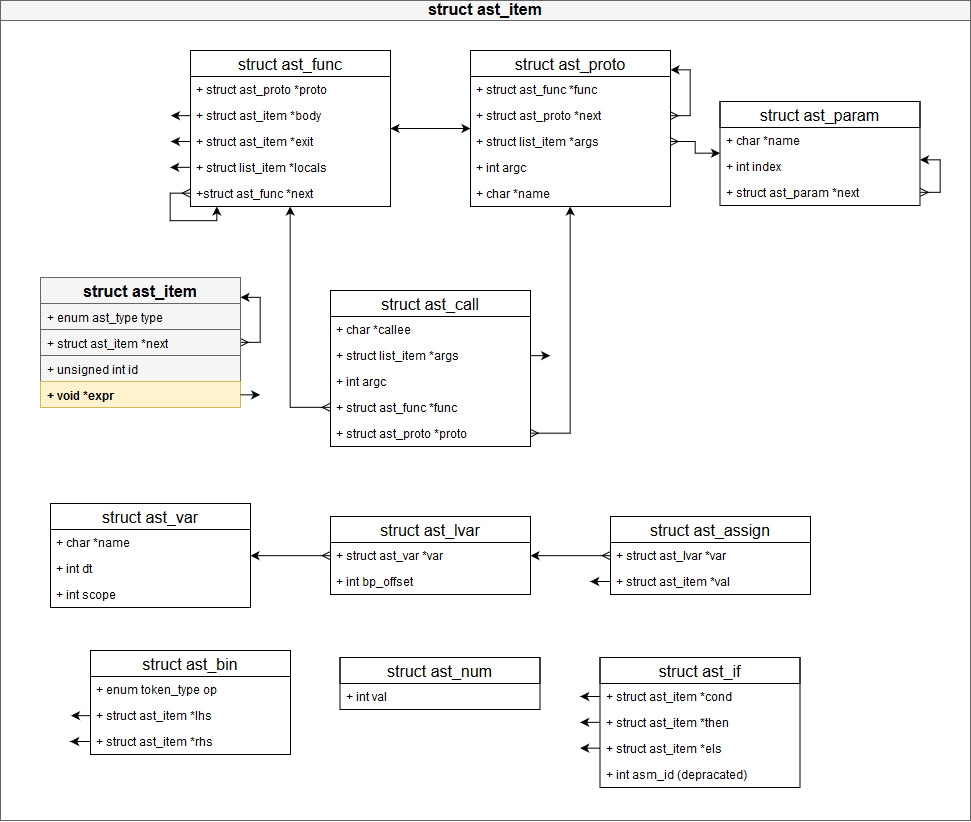
\includegraphics[scale=0.4]{compiler_ast_item}
\end{center}
\caption{UML class diagram showing the AST structures and their connections. The \mintinline{C}{struct ast_item} structure is a top level structure that contains pointers to specific AST items (such as \mintinline{text}{ast_func} and \mintinline{text}{ast_lvar}). It is a self-referencing structure and can be iterated over in a linked-list using it's \mintinline{text}{*next} property using the provided macro: \mintinline{text}{list_for_each()}. It can be thought as a generic header for each AST type allowing it to be passed as a \mintinline{text}{void*} and still identified through it's \mintinline{C}{enum ast_type type} parameter.}
\label{fig:compiler_ast_uml}
\end{figure}



\subsection{Optimisation}
The \scname{} compiler can optionally perform simple optimisations, such as unreachable code elimination and constant folding. The optimisations can be controlled by specifying the \verb|-On| parameter to the CLI, where \verb|n| is the level of optimisation.

The techniques used by the optimiser to perform these optimisations are primitive; the optimiser is not given AST information in SSA (static single assignment) form; and because of this limitation, only basic optimisations can be identified.

\subsubsection{Constant Folding}
Constant folding is performed by the optimiser to reduce (fold) expressions that can be identified as constant. This allows the optimiser to replace AST tree structures containing constant values and no dependencies with shorter and simpler AST items. This optimisation can drastically improve the performance of the output code by reducing the number of instructions emitted.

For example, the following expression in Figure \ref{fig:constant_fold_yes} can be identified as constant and can be reduced to a single AST node as shown in Figure \ref{fig:constant_fold_ast}. As the optimiser is not passed AST information in SSA form, the optimiser cannot follow or track variable references and modifications throughout the life-cycle of the program. Although the parser does a contain a primitive symbol table, the symbol table does not map variables to values, and so the code segment in Figure \ref{fig:constant_fold_no} cannot be identified as constant by the optimiser.


\begin{figure}[H]
\centering 
\begin{minipage}{0.4\textwidth}
\begin{minted}{C}
int a = 1 + (2 + 3) * 4;
\end{minted}
\end{minipage}
\caption{Example of an expression suitable for constant folding.}
\label{fig:constant_fold_yes}
\end{figure}

\begin{figure}[H]
\centering 
\begin{minipage}{0.4\textwidth}
\begin{minted}{C}
int a = 1;
int b = 2;
int c = a + b;
\end{minted}
\end{minipage}
\caption{Example of an expression the optimiser cannot identify as constant.}
\label{fig:constant_fold_no}
\end{figure}

\begin{figure}[H]
%\begin{wrapfigure}{r}{0.6\textwidth}
\begin{center}
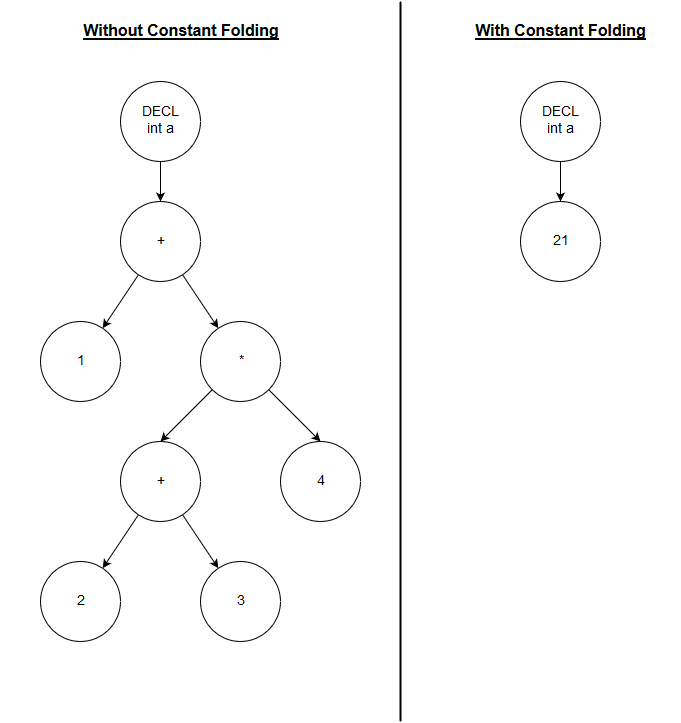
\includegraphics[scale=0.4]{compiler_cf}
\end{center}
\caption{AST transformation performed by Constant Folding.}
\label{fig:constant_fold_ast}
\end{figure}
%\end{wrapfigure}
%\lipsum[1]
%\lipsum[1]



\subsubsection{Unreachable Code Elimination}
Unreachable code elimination is the removal of code that will never be run on the processor. This can be in the form of uncalled function, unused variables, and control statements that operate on constant values.

The \scname{} compiler can identify some unreachable code segments, such as control statements that operate on constant values, by utilising it's constant folding optimisation discussed previously. By first running the constant folding optimisation on the body of functions, the optimiser looks at the conditions of \textit{if} statements. If it's condition has been constant folded to a constant and is \textit{true} (i.e. not 0) then the AST tree can be replaced with the items in it's body, effectively removing the condition check if it's always true, or the whole structure if it's false.

\subsection{Code Generation}
The compiler Code Generation stage converts the optimised AST into an intermediatary list of \mintinline{c}{struct prco_op_struct}. It does this by iterating over each \mintinline{c}{struct ast_item} in the AST and checks whether the item requires code generation. For example, an \mintinline{c}{struct ast_item} with type \mintinline{c}{AST_FUNC} is one which requires code generation. The AST is then passed to the \mintinline{c}{void cg_func_prco(...)} function where the code generation takes please. For this type, the stack frame header is generated first, before the body of the function. At the end of the function's body, the stack frame end code generation routing is run.

This code generation stage is named intermediatary because absolute addresses of \verb|JMP| instructions have not been calculated. The calculation of these addresses is performed in the following Assembling stage. In addition, the location (and offset's) of functions may need to be rearranged.

\subsubsection{Variables}
\label{sect:compiler_cg_vars}
An initial requirement for the \scname{} compiler was to support three types of variables: global, local, and parameter variables. Due to time constraints and unforeseen \textit{"sleeper"} bugs only local and argument variables have been implemented as of compiler version 2.50 (06/04/2018). Global variable allocation has been implemented in the assembler but declaring or referencing global variables has not been implemented.

\subsubsection*{Local Variables}
Similar to C89, all local variables must be declared at the start of the function before any logic, such as function calling. This is because the compiler will not rearrange the AST tree to move variable declarations to the first child of the function AST tree.

When a local variable is declared, stack space is immediately allocated for the variable by subtracting the data type size (1 word) from the Base Pointer variable. Although the code generator knows how many local variables are in a function, due to time constraints, it will not reduce/fold multiple stack allocations into a single SUBI instruction. The output machine code looks similar to Figure \ref{fig:compiler_cg_lvars} below.

\begin{figure}[!h]
    \begin{minipage}{0.5\textwidth}
        \centering
\begin{minted}[linenos]{text}
MOV   %Bp, %Sp     1ee0 (STACK FRAME)
SUBI  %Sp, $1      5f01 (ALLOC a -3)
SUBI  %Sp, $1      5f01 (ALLOC b -2)
SUBI  %Sp, $1      5f01 (ALLOC c -1)
LW    %Ax, -3(%Bp) 08dd (REF a -3)
LW    %Ax, -2(%Bp) 08de (REF b -2)
LW    %Ax, -1(%Bp) 08df (REF c -1)
\end{minted}
        \captionof{figure}{Disassembly of the output machine code for the high-level code (\ref{fig:compiler_cg_lvars_high}).}
        \label{fig:compiler_cg_lvars_asm}
    \end{minipage}
    \begin{minipage}{0.05\textwidth}\hfill\end{minipage}
    \begin{minipage}{0.5\textwidth}
        \centering
\begin{minted}[linenos]{c}
fnc main() {
    int a; int b; 
    int c;
    a; b;
    c;
}
\end{minted}
        \captionof{figure}{Input high-level code showing 3 variable declarations and references.}
        \label{fig:compiler_cg_lvars_high}
    \end{minipage}
    \captionof{figure}{Example machine code generation for local variables.}
    \label{fig:compiler_cg_lvars}
\end{figure}

Variables are then accessed using the \verb|LW| instruction and passing a 5-bit signed immediate constant as seen above.

\subsubsection*{Argument Variables}
The compiler uses a modified implementation of the \verb|stdcall| calling convention \cite{callconv}. The difference is that arguments are pushed \textit{left to right} instead of \textit{right to left}. This difference is due to limited time constraints and was made worse by the use of a singly-linked list for storing arguments, which made list reversal time consuming. The compiler overcomes this difference by reversing variable offset addresses of the parameters of the function. The affect of this implementation might cause externally compiled programs to be incompatible with programs compiled with this \scname{} compiler. This is easily solvable by reversing the argument list before pushing.

Figure \ref{fig:compiler_cg_vars_args} below shows the code generation routine used by the compiler to push function call arguments to the stack before jumping to the function.

\begin{figure}[H]
\centering 
\begin{minipage}{0.4\textwidth}
\begin{minted}[
    linenos,
    firstnumber=628]{c}
args = c->args;
list_for_each(args) {
    cg_expr_template(args->value);
    cg_push_prco(Ax);
}
\end{minted}
\end{minipage}
\caption{Code generation routine for pushing arguments to the stack before the function call. (\textit{arch/template\_impl.c:628})}
\label{fig:compiler_cg_vars_args}
\end{figure}


\subsubsection*{String Variables}
Strings are an extended deliverable for the \scname{} compiler but was added to better demonstrate the capabilities of the compiler and processor. Strings in modern OS executable file formats, such as ELF \cite{elf_standard} and Windows' PE \cite {winpe_standard}, store explicitly declared strings as null-terminated ASCII (ASCIZ) strings in the String Table or \verb|.text| section of the executable file.

The \scname{} processor places strings and global values at the start of low memory. As the processor starts executing instructions at address \verb|0x00|, the compiler must insert a jump instruction to the address of the \verb|main| function.

A limitation in memory addressing and storage within the \scname{} processor prevents memory cells being indexed at byte boundaries. Due to limited time, it was decided with the project supervisor to store each byte character in a 2-byte cell. This keeps the functionality but reduces memory density.

\begin{figure}[H]
    \begin{minipage}{0.5\textwidth}
        \centering
\begin{minted}[linenos]{text}
0x00 MOVI   $6,  Bx  2106 (ENTRY)
0x01 JMP    Bx,  JUC 6100 
0x02 ASCII  b    1   0062 
0x03 ASCII  e    0   0065 
0x04 ASCII  n    0   006e 
0x05 ASCII       0   0000 
0x06 ADDI   $-1, Sp  4fff (FUNC)
\end{minted}
        \captionof{figure}{Disassembly of the output machine code for the high-level code. Local variable declaration '\textit{a}' is assigned the value \textit{0x02} which is the address of the first byte of the ASCIZ string.}
        \label{fig:}
    \end{minipage}
    \begin{minipage}{0.05\textwidth}\hfill\end{minipage}
    \begin{minipage}{0.5\textwidth}
        \centering
\begin{minted}[linenos]{c}

fnc main() 
{
    int a = "ben";
    
    ...
}
\end{minted}
        \captionof{figure}{Input high-level code showing a string variable declaration.}
        \label{fig:}
    \end{minipage}
    \captionof{figure}{Example machine code generation for string variables.}
    \label{fig:compiler_cg_strings}
\end{figure}

\subsubsection*{Pointers and Value Dereferencing}
With the implementation of string variables, the concepts of pointers and dereferencing is implicitly introduced. 
\begin{figure}[H]
    \begin{minipage}{0.5\textwidth}
        \centering
\begin{minted}[linenos]{c}
void strlen() {
    char *str = "testing";
    int length = 0;
    
    while( *(str + length) ) {
        length++;
    }
    
    printf("%d", length);
}
\end{minted}
        \captionof{figure}{C function to calculate the length of a string and print to console.}
        \label{fig:compiler_cg_vars_asm}
    \end{minipage}
    \begin{minipage}{0.05\textwidth}\hfill\end{minipage}
    \begin{minipage}{0.5\textwidth}
        \centering
\begin{minted}[linenos]{c}
fnc strlen() {
    int str = "testing";
    int length = 0;

    while( @(str + length) ) {
        length = length + 1;
    }

    UART1(length + 48);
}
\end{minted}
        \captionof{figure}{Equivalent function to print the length of a string to UART in the \scname{} programming language.}
        \label{fig:compiler_cg_vars_high}
    \end{minipage}
    \captionof{figure}{Example machine code generation for value dereferencing.}
    \label{fig:compiler_cg_vars}
\end{figure}



\subsection{PUSH and POP}
\label{sect:compiler_cg_push_pop}
PUSH and POP concepts are a simple yet powerful method in computer architectures to support complex, nested, and recursive functionality, such as function calling and parameter passing.

Due to limitations of the \scname{} processor's instruction set, high-level instructions such as PUSH and POP cannot be performed in a single instruction as with architectures like x86 and ARM's Thumb2. With discussion with the project supervisor, it was decided to replicate the behaviour of these high level instructions by emitting multiple primitive instructions. Figure \ref{fig:compiler_cg_push_pop} below details how the compiler emulates these high-level instructions.

\begin{figure}[H]
    \begin{minipage}{0.5\textwidth}
        \centering
        \begin{minted}{c}
void cg_push_prco(enum prco_reg rd)
{
    asm_push(opcode_add_ri(Sp, -1));
    asm_push(opcode_sw(rd, Sp, 0));
}
        \end{minted}
        \captionof{figure}{PUSH emulation. The Stack Pointer is subtracted the amount to store on the stack (1 word), followed by storing the destination register (\textit{rd}) at the new Stack Pointer.}
    \end{minipage}
    \begin{minipage}{0.01\textwidth}\end{minipage}
    \begin{minipage}{0.5\textwidth}
        \centering
        \begin{minted}{c}
void cg_pop_prco(enum prco_reg rd)
{
    asm_push(opcode_lw(rd, Sp, 0));
    asm_push(opcode_add_ri(Sp, 1));
}
        \end{minted}
        \captionof{figure}{POP emulation. The value pointed to by the Stack Pointer is loaded in the destination register (\textit{rd}), followed by incrementing the Stack Pointer the size of the data type (1 word).}
    \end{minipage}
    \captionof{figure}{PUSH and POP emulation functions used by the \scname{} compiler (\textit{arch/prco\_impl.c:255}). Example of use:
    \mintinline{C}{cg_push_prco(Ax)} to push register Ax to the stack; \mintinline{C}{cg_pop_prco(Ax)} to pop stack into Ax.}
    \label{fig:compiler_cg_push_pop}
\end{figure}



\section{Assembling}
The final stage of the compiler is the assembling stage. This stage takes the list of \mintinline{c}{struct prco_op_struct} and outputs a list of machine code instructions. The assembler accomplishes this by calculating offsets and addresses of functions, branching instructions, and global variable addresses. It may also rearrange function locations so that the main function is the first instruction to be emitted.

Assembling code is found in \verb|assembler_labels()| at \verb|arch/template_impl.c:38|.

\subsection{Executable Layout}

\begin{figure}[H]
%\begin{wrapfigure}{r}{0.3\textwidth}
\begin{center}
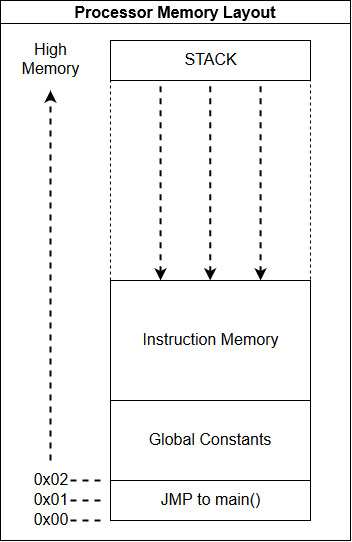
\includegraphics[scale=0.4]{prco_memory_layout}
\end{center}
\caption{\scname{} memory layout showing Global, Instruction, and Stack memory sections.}
\label{fig:asm_mem_layout}
%\end{wrapfigure}
\end{figure}

Another role of the assembler in the \scname{} processor is to output the machine code in a format that allows the widest range of programs to be run by the processor.

This format is not enforced by the processor core and it's up to the compiler to lay out the processor's memory contents. The only feature that the processor states is that it will start reading instructions from address \verb|0x00|. The compiler uses this information to structure the output program. The first two words of memory (\verb|0x00| and \verb|0x01|) contain \verb|MOVI| and \verb|JMP| instructions to jump the processor to the address of the \verb|main()| function.

\subsection{Address Limitations}
Due to time constraints, the assembler introduces many constraints to the output program that are not explicitly identified in the high-level code.

The most prominent limitation is that the assembler can only address 256 words of memory. This is because the assembler only builds up instruction addresses using a single MOVI instruction, which is limited to an 8-bit immediate. This is easily fixable as the assembler could insert additional instructions to build up 16-bit addresses to use. For example, to build a 16-bit address, \textit{0xFECA}, the following instructions could be used (move \verb|0xFE| into \verb|Ax| and shift left 8-bits, then \verb|OR| it with \verb|0xCA| to make \verb|0xFECA|):
%TC:ignore
\begin{minted}{asm}
MOVI  $0xFE,   %Ax
LSHF  %Ax,     $8
ORI   %Ax,     $0xCA
JMP   %Ax,     JE_UC (unconditional)
\end{minted}
%TC:endignore
This is described in GitHub issue \href{https://github.com/bendl/prco304/issues/20}{\#20}.

\section{Testing and Verification}
Verifying the output assembly is a bit more involved as there are multiple layers of tests required. The output code generation must be tested for:
\begin{itemize}
\item{(A) Correct instruction and machine code building.}
\item{(B) Correct instruction sequences for different code generation routines.}
\item{(C) Correct and complete flow of the output program and any divergent paths.}
\end{itemize}

\subsection*{Unit Testing}
For (A) and (B), a code generation routine refers to the code generation function used to produce machine code for a specific structure, for example a function or assignment expression. When machine code instructions are emitted from the code generation routines, they are pushed to a list of \mintinline{c}{struct prco_op_struct} containing information about the emitted instruction. Using this information, the final output machine code word (e.g. \mintinline{c}{0x2020}) is rebuilt into an equivalent \mintinline{c}{struct prco_op_struct} structure and compared against the original. If they are the same, the encoded machine code word is considered correct. This check happens every time an instruction is emitted from the code generation routines.

\subsection*{Real Hardware Tests}
The \textit{best} approach to verifying output machine code is to run it directly on the \scname{} processor. However, this requires rebuilding the FPGA design with the new program code which is time consuming and not always practical. In addition, viewing of internal registers and signals is much more difficult due to the lack of a debugging interface on the processor.
 
\subsection*{Emulation}
During the later stages of the project, it was decided to build a software emulator for the \scname{} processor. The emulator, found at \verb|prco_compiler/emu/emu.c|, would utilise structures used in the compiler's assembling stage to rebuild instructions and their contents from raw machine code words. The emulator aims to replicate the structure and design of the embedded processor: on-chip memory, registers, complex ALU operations such as CMP, JMP, and SETC, and UART.

Due to the late development of the emulator, and it not being a deliverable, and only developed as an alternate means to test the processor, the emulator is not a full emulation of the processor. The emulator implements most features of the processor, including registers, memory, ALU operations, and most instructions. It is capable of emulating all the test programs (found in \verb|proc_compiler/tests/*.prco|).

With the introduction of the emulator, the process of deploying high-level code changed from: \textbf{write, compile, deploy, verify, repeat}; to \textbf{write, compile, emulate, verify, repeat, deploy, verify}. By reducing the number of deploys, time taken to successfully write working code was drastically improved.

Late in the project, the ability of integrating the emulator into unit tests for the compiler was completed. This allowed for fast and more complete verification of the compiler that could verify multiple programs on every code change.

\subsection*{Continuous Integration}
The \scname{} compiler employs continuous integration testing to show if a code commit breaks certain functionality. The continuous integration system service used is Travis CI \cite{travisci}. Every time a commit is made to the repository, Travis CI pulls the commit and runs the \verb|test/travis-ci.sh| script. This script runs the compiler and emulator on each \verb|test/*.prco| file and checks the return code. If the return code does not match the expected functionality, the test fails and the developer can investigate further by enabling more debug prints with the \verb|-D| parameter. These tests will generate a report detailing passed and failed tests with their actual and expected outputs. 

This method accomplishes verification requirement (C). By running automatic tests for each code change, it allows the developer to quickly identify bugs. In addition, running all tests for any code change allows the developer to identify changes that unknowingly affect other parts of the program. This continuous integration testing methodology greatly aids the end-user in their goal of bug-free code compilation.

An example output of the continuous integration test runner is located in section \ref{appendix:travisci} {\nameref{appendix:travisci}}. The continuous integration results can be viewed here: \url{https://travis-ci.com/bendl/prco304/}.

\newpage
\section{\scname{} Compiler Review}
This section reviews the design, implementation, verification, and management of the \scname{} compiler project.

\subsection{Functional Requirements}
All functional requirements, (F1 - F7), have been achieved. 

\subsection{Core Compiler Components}
\begin{table}[H]
\def\arraystretch{1.3}
\caption{Compiler Core Deliverables Review}
\begin{tabularx}{\textwidth}{|p{4cm}|c|c|X|}
\hline 
Deliverable & Implemented & Version & Comment \\ 
\specialrule{2pt}{-2pt}{0pt}
CFG Text Parser & Yes & 1.00 & Recursive descent parser.\\ 
\hline 
AST Intermediate Representation & Yes & 1.00 & \\ 
\hline 
Basic arithmetic Operators & Yes & 1.10 & Features operator precedence. \\ 
\hline 
IF statements 	& Yes & 1.30 & \verb|if ( <expr> ) { ... }| \\ \hline 
IF ELSE statements & Yes & 1.30 & \verb|if ( <expr> ) { ... } else { ... }|. Else must be followed by an opening bracket character so no \verb|else if| statements, although you can nest them instead. \\ \hline 
FOR statements 	& Yes & 1.30 & Similar syntax to C's for loop.\\ \hline 
Functions	 	& Yes & 1.20 & Stack frame creation for each function allows for recursive and nested calling. \\ \hline 
Variables 		& Limited & 1.50 & Only local and argument variables. No global variables.\\ \hline 
Code generation & Yes & 1.30 & Output is presented to the user in both machine code and assembly-like text.\\ \hline
Assembling 		& Yes & 1.40 & Basic offset calculation and instruction re-encoding.\\ 
\hline 
\end{tabularx} 
\end{table}


\subsection{Extended Compiler Components}
\begin{table}[H]
\def\arraystretch{1.0}
\caption{Compiler Extended Deliverables Review}
\begin{tabularx}{\textwidth}{|p{4cm}|c|c|X|}
\hline 
Deliverable & Implemented & Version & Comment \\ 
\specialrule{2pt}{-2pt}{0pt}
Assembly text parsing & No & X & Only the CFG text parser for the grammar described in section \ref{sect:compiler_grammar} is present. This would be a desirable feature for implementing features the compiler is not able to.
\\ \hline 
Optimisation: Constant Folding & Yes & 2.00 & Limited to compile time constants. 
See \verb|prco_compiler/libprco/opt.c:9|. \\ \hline 
Optimisation: Unreachable-code elimination & Yes & 2.00 & Limited to IF statement constants. 
See \verb|prco_compiler/libprco/opt.c:33|. \\ \hline
String variables      & Limited & 2.10 & All strings are placed in low memory, not on stack. Limited to alphanumeric identities (easily fixable).\\ \hline 
Dereferencing         & Yes & 2.10 & Uses low precedence \verb|@| symbol. Unsafe like C's \verb|*| dereferencing functionality. See \verb|prco_compiler/test/tests/control_for_3.prco|. \\ \hline 
\textit{Pointer} arithmetic & Yes & 2.10 & Inferred by dereferencing implementation. 
E.g. \verb|@(a+1)| returns contents of memory address at value \verb|a+1|. 
\\ \hline 
Assembler memory layout & Yes & 2.10 & First instructions (low memory) jump into \textit{middle} memory where \verb|main| function is located. Low memory consists of \textit{global values} (like strings and global variables). High memory is reserved for stack management. 
\\ \hline 
\end{tabularx} 
\end{table}

\chapter{End-Project Report}
{\hypersetup{linkcolor=black}
\startcontents[chapters]
\printcontents[chapters]{}{1}{}
}

\section{Project Objectives}
\begin{description}[style=nextline]
\item [C1. To improve my knowledge and experience of FPGA development, processor architecture, compilers, and embedded systems engineering.]

This primary objective has been accomplished. The combination of the initial research into existing embedded processors and compilers and applying that knowledge to design a new architecture and it's implementation on FPGA devices. 

Debugging on live FPGA devices is challenging and so sufficient verification must be performed prior to deployment. This has gained me a lot of experience in troubleshooting FPGA designs in simulation and when implemented on the device.

The compiler development has taught me how to transform target-independent code, firstly to multiple immediate representations, and then finally to target-dependant implementations.

\item[C2. To build a working and operational soft-core processor core capable of performing simple tasks.]
The first half of this project was to design, implement, and verify an embedded processor. The processor was designed in Verilog, a hardware description language. Modularised components were written, such as the decoder, register set, and ALU, and connected with control signals to implement a simple data pipeline. 

Once the processor was able to support a program counter, instructions could be fetched, executed, data written, and control execution of the processor. With the addition of comparison and branching instructions, CMP and JMP, dynamic execution and program flow was introduced. This allows the processor, without knowledge of high-level concepts such as \textit{if} and \textit{for} loop statements, to perform complex logic sequences by executing primitive instructions.

With the aid of the compiler, tasks such as multiplication, division, string manipulation, and variables, complex tasks are more easily accomplished. In addition, the inclusion of a UART interface allows the processor to send data externally. The UART output can be connected to other devices as a UART input to share data, for example printing text to an RS232 shell.

\item[C3. Implementation of the soft-core processor design on real hardware (FPGA).]
A large risk of the project, \ref{risk:hw} to implement the Verilog processor on an FPGA device, specifically the MiniSpartan-6+ XC6SLX9 development board (\ref{res:minispartan}), had appeared throughout development of the processor. As stated in the {\nameref{pid}}, issues like this occur when synthesised HDL code does not meet the physical constraints of the device (in our case, an FPGA). This results in different behaviour between simulation and hardware which is a critical problem. 

This issue was reduced by enabling warnings during ISE's synthesis and place-and-route tools of the HDL code to the FPGA device. When these warnings were present, the respective code was redesigned in order to meet the device's constraints.

As discussed in section {\nameref{ise_impl}}, the \scname{} processor has been successfully implemented on the MiniSpartan6+ development board. Although successful, the implementation did take up more FPGA slice resources, likely caused by poorly designed register and RAM components that did not infer to physical FPGA block RAMs. This would result in smaller FPGA logic space available to the developer.


\item[C4. To provide a high-level context-free code compiler to run user-code on the processor.]
A C-like grammar compiler was designed, implemented, and verified. The compiler accepted a context-free grammar similar to C's grammar. The grammar featured terminal symbols for variables and arithmetic operators, and non-terminal  symbols for complex patterns like \textit{for} loops and function definitions.

The compiler would represent this input grammar in an abstract syntax tree structure. This structure allowed for easy rearrangement and modification for optimisations to be performed. Simple optimisations like constant-folding and dead-code elimination were implemented.

The compiler successfully output machine code in a format accepted by the \scname{} processor. Example programs were provided showing implementation of simple tasks, such as string length finding, variables, and UART transmitting.
\end{description}

\newpage
\section{Project Post-mortem}
\subsection*{Research and Requirements Elicitation}
Due to the high complexity of the project and availability of existing processor designs, I was able to easily find thoroughly documented processor designs and specifications. These are normally in the form of developer-facing technical manuals which detail the operation and characteristics of the processor. By reading multiple processor specifications, I quickly built up an understanding of existing processor designs and how they are technically presented to developers to integrate into their own projects. The application of this knowledge can be seen throughout this project: the \scname{} processor high-level design; and the ISA.

\subsection*{Development Process}
The combination of PRINCE2 with Agile was a success. The alignment of Agile's sprints and PRINCE2's highlight reports and stages made developing the project easier. A Kanban board was created to track stages, requirements, and bugs, and to  organise and present them clearly. In addition, milestones were created allowing tasks to be better scoped.

\subsection*{Technology Review}
Using LaTex for all documentation aided the project greatly. LaTex, being a text-based document editor, worked great when combined with version control, such as Git. This allowed for easier tracking, reviewing, and merging of document changes throughout the project. Although requiring an initial learning curve, however once passed, documents could be edited quickly and professionally with skill.

Verilog was chosen for the processor code development. Other HDL languages were available, such as VHDL, but my experience with those is negative; little documentation and varying quality resources for learning. Verilog, is also closer to C than VHDL, which makes learning and writing the language easier to transition too. Although Verilog will implicitly transform code, such as register length conversions, I did not find this to be an issue and the processor core worked as designed.

C was used for the compiler and emulator. Higher level languages could have been used for the same result, such as Python, but these would have abstracted away important concepts used by compilers, such as AST transformations, and optimisations. In addition, I am most proficient in C than other sequential programming languages. OOP concepts were avoided as they would introduce too much complexity and negatively affect the projects forward-compatible design. Overall, C was a good choice for the compiler and emulator.

\subsection*{Personal Contribution Review}
I am pleased with the outcomes of this project and my contributions to it. I wanted to improve my knowledge and experience with FPGAs, computer architecture, and low-level programming, and so a project requiring these skills was developed. Easier technologies could have been used (for example, Python for the compiler), but this would have abstracted important processes, such as AST transformations and instruction encoding, away from me resulting in less experience gained.

Throughout this project, I have learnt and improved upon my Verilog and C programming skills as well as learning new debugging techniques, such as HDL simulation and emulation.

\subsection*{Changes}
The project has utilised agile development to review and introduce unseen features as needed. For example, the need for a new instruction SETC was identified and was introduced in the project, as well new ISA types for special instructions. 

As seen in the highlight reports, there was originally planned to provide a processor documentation guide. Due to time constraints however, this document has been split up merged into the Report and Appendix. It originally featured content about the ISA and pipeline.


\subsection*{Future Improvements}
This was my first attempt at a compiler capable of generating and assembling machine code and an embedded FPGA-based processor. Although much as been learned, the design and implementation shows that a number of improvements can be made. Firstly, the design of the processor's pipeline was not parallel, meaning that only 1 instruction could be fetched, executed, and written to, at any time. This was because the processors components (decoder, registers, RAMs), used global wires connecting them, instead of a wires connecting them from module to module. This would enable a scalar pipeline to be implemented.

The compiler was only able to transform high-level code into machine code. Even though the compiler would display assembly like code representing the machine code, users could not write or compile it; it was merely there to help debug the generated code by making it easier to read the machine code. Enabling parsing of assembly like code would enable specific routines to be created which would enable more complex applications to be created, such as operating system kernels and reliably timed routines.

It was found that the implemented processor was difficult to debug and troubleshoot. This is an important problem in FPGA-based products. A common solution employed in processors and FPGA-based products is to employ a debugging interface in the design, such as JTAG or other scoped-buses. This would be too timely to fit into this projects timeline, but will be crucial if complex features are to be added to the processor.

\newpage
\section{Conclusion}
This project aimed at producing two complex technical systems: an embedded processor and a compiler. Both systems were developed and the output is an extremely valuable educational resource. 

The technologies created from this project spawning from the compiler include:
\begin{itemize}
\item{an easily extendible recursive-descent text parser;}
\item{an AST optimiser for constant-folding and unreachable code elimination;}
\item{a machine code generator and assembler;}
\item{and an emulator (not originally planned, but was a key tool required later in the project).}
\end{itemize}
And from the embedded processor:
\begin{itemize}
\item{a 16-bit instruction set and it's implementation;}
\item{and a feed-forward pipeline architecture.}
\end{itemize}

A wide-range of test programs were written that implement common programming features such as \verb|for| and \verb|while| loops, functions, and variables. These features are combined to perform general and complex programs such as string length finding, UART printing, and variable modification. From the range of these test programs, it clearly shows the potential of the processor and compiler and it's ability to perform a wide range of programs. 

I believe these technologies and their implementation details should be shared as an open, educational resource for future projects and people interested in low-level code generation and embedded processor architecture.






\newpage
\bibliography{prco304}


\newpage
%TC:ignore
\chapter{Appendices}
\linespread{1.0}
{\hypersetup{linkcolor=black}
\startcontents[chapters]
\printcontents[chapters]{}{1}{}
}

\section{Appendix A. User Guides}
\subsection{\scname{} Core Reference Guide}
\subsubsection*{Instantiating the core in your FPGA design}
The \scname{} processor core can be instantiated in an FPGA design with the following code snippet:
\begin{minted}{verilog}
// Instantiate a processor core
prco_core inst_core (
    .i_clk(), 
    .i_en(), 
    .i_reset(),
    
    // Operating mode (HIGH=single-step)
    .i_mode(),
    // Single-step pulse
    .i_step(),
    
    // UART comms
    .i_rx(),
    .q_tx(),
    .q_tx_byte(),
    
    // Debug outputs
    .q_debug_instr_clk(),
    .q_debug()
);
\end{minted}


\subsection{\scname{} Compiler Reference Guide}
\subsubsection*{Building the Compiler}
To build the compiler (\verb|cli| front-end and \verb|libprco| back-end), run the following commands:
\begin{minted}{bash}
cd prco304
mkdir build && cd build
cmake ..
cmake --build .
\end{minted}
If you wish to build the compiler's own standard library run the following command as root/administrator to install the sources and header files:
\begin{minted}{bash}
cmake --build . --target install
\end{minted}

\subsubsection*{Command Line Interface (CLI) Arguments}
\label{sect:compiler_cli}
\begin{description}[style=nextline]
\item [Name]
\verb|cli| - compile a program into executable machine code for the \scname{} processor.

\item[Synopsis]
\verb|cli [OPTION]... -i{FILE}|

\item [Description]
\verb|-d| Dump output machine code to a file

\verb|-D{bits}| Select debug printing level. Example of use: \verb|-D0xFF| to enable all debug bits. 

\verb|-i{file}| Pass the input file to the compiler. Example of use: \verb|-i code.prco|.

\verb|-O{0-1}| Enable optimisation levels. \verb|0| = no optimisations, \verb|>0| = constant folding and unreachable code elimination.

\verb|-m{arch}| Pass the target architecture to the compiler. Deprecated.

\end{description}


\subsection{\scname{} Emulator Reference Guide}
\label{sect:emulator_cli}
\begin{description}[style=nextline]
\item [Name]
\verb|emu| - Disassemble and emulate \scname{} processor programs.

\item[Synopsis]
\verb|emu [OPTION]... -i{FILE}|

\item [Description]
\verb|-i| Input machine code file. 1 instruction word per line. CRLF/LF accepted.

\verb|-D{bits}| Select debug printing level. Example of use: \verb|-D0xFF| to enable all debug bits. 
\end{description}


\subsection*{Example Output}
\inputminted{text}{emu_output.tex}
\scriptsize
The output of the emulator starts with the disassembly of the processors input. As the instructions are reconstructed from the 16-bit instruction words, we lose additional information displayed by the compiler when this program was originally compiled, such as inline comments explaining the code-generation routine used (last column) and any assembler tags (second-last column) used by the assembler (see \textit{libprco/arch/prco\_isa.h:72}).

Next follows the initial memory layout of the processor. This shows where each instruction word is placed in memory. The emulator limits the displayed memory to the first 255 words of memory.

Following this is the list of executed instructions. Instruction execution starts at PC  (program counter) \verb|0x00|. On the right side, the contents of each memory is displayed. For complex instructions such as \verb|LW/SW| and \verb|WRITE| additional information is printed to verify correct ALU operation.
\normalsize

\subsection{\scname{} Compiler Continuous Integration Tests}
\label{appendix:travisci}
\inputminted{text}{compiler_ci.txt}

\newpage
\subsection{\scname{} Processor Instruction Set Architecture}
\label{appendix:isa}

\subsubsection*{NOP}
\label{isa_nop}
\begin{description}[align=right,labelwidth=4cm]
\item [Description] The NOP instruction performs no action for 1 instruction cycle.
\item [Assembly] NOP
\item [Pseudocode] PC $<$= PC + 1;
\item [Registers altered] None
\item [Clock cycles] 2 (FETCH, DECODE)
\end{description}

\begin{table}[h]
\def\arraystretch{1.3}%  1 is the default, change whatever you need
    \begin{tabularx}{\textwidth}{|p{4cm}|X|}
    \hline
    15:11 & 10:0 \\
	\specialrule{2pt}{-2pt}{0pt}
	00000 & X
	\\ \hline
    \end{tabularx}
\end{table}


\subsubsection*{LW - Load Word}\label{isa_lw}
\begin{description}[align=right,labelwidth=4cm]
\item [Description] Copies a 16-bit word from RAM to a register.
\item [Assembly] LW Rd, +4(Ra)
\item [Pseudocode] Rd $<=$ RAM[Ra + Simm5]
\item [Registers altered] Rd
\item [Clock cycles] 6 (FETCH, DECODE, READ, EXECUTE, RAM, WRITE)
\end{description}

\begin{table}[H]
\def\arraystretch{1.3}%  1 is the default, change whatever you need
    \begin{tabularx}{\textwidth}{|p{4cm}|p{2cm}|p{2cm}|X|}
    \hline
    15:11 & 10:8 & 7:5 & 4:0 \\
	\specialrule{2pt}{-2pt}{0pt}
	00001 & Rd & Ra & Simm5
	\\ \hline
    \end{tabularx}
\end{table}


\subsubsection*{SW - Store Word}\label{isa_sw}
\begin{description}[align=right,labelwidth=4cm]
\item [Description] Copies a 16-bit from a register to RAM.
\item [Assembly] SW Rd, +4(Ra)
\item [Pseudocode] RAM[Ra+Simm5] $<=$ Rd
\item [Registers altered] None
\item [Clock cycles] 6 (FETCH, DECODE, READ, EXECUTE, RAM, WRITE)
\end{description}

\begin{table}[H]
\def\arraystretch{1.3}%  1 is the default, change whatever you need
    \begin{tabularx}{\textwidth}{|p{4cm}|p{2cm}|p{2cm}|X|}
    \hline
    15:11 & 10:8 & 7:5 & 4:0 \\
	\specialrule{2pt}{-2pt}{0pt}
	00001 & Rd & Ra & Simm5
	\\ \hline
    \end{tabularx}
\end{table}

\subsubsection*{MOVR}
\begin{description}[align=right,labelwidth=4cm]
\item [Description] Copies a 16-bit register value to another register.
\item [Assembly] MOVR \%Ra, \%Rd 
\item [Pseudocode] Rd $<=$ Ra
\item [Registers altered] Rd
\item [Clock cycles] 5 (FETCH, DECODE, READ, EXECUTE, WRITE)
\end{description}

\begin{table}[H]
\def\arraystretch{1.3}%  1 is the default, change whatever you need
    \begin{tabularx}{\textwidth}{|p{4cm}|p{2cm}|p{2cm}|X|}
    \hline
    15:11 & 10:8 & 7:5 & 4:0 \\
	\specialrule{2pt}{-2pt}{0pt}
	00011 & Rd & Ra & X
	\\ \hline
    \end{tabularx}
\end{table}

\subsubsection*{MOVI}\label{isa_movi}
\begin{description}[align=right,labelwidth=4cm]
\item [Description] Copies an 8-bit immediate to a Register
\item [Assembly] MOVR \%Ra, \%Rd 
\item [Pseudocode] Rd $<=$ Imm8
\item [Registers altered] Rd
\item [Clock cycles] 5 (FETCH, DECODE, READ, EXECUTE, WRITE)
\end{description}

\begin{table}[H]
\def\arraystretch{1.3}%  1 is the default, change whatever you need
    \begin{tabularx}{\textwidth}{|p{4cm}|p{3cm}|X|}
    \hline
    15:11 & 10:8 & 7:0 \\
	\specialrule{2pt}{-2pt}{0pt}
	00100 & Rd & Imm8
	\\ \hline
    \end{tabularx}
\end{table}


\subsubsection*{ADD}
\begin{description}[align=right,labelwidth=4cm]
\item [Description] Add the value of register Ra to Rd.
\item [Assembly] ADD \%Rd, \%Ra
\item [Pseudocode]Rd $<=$ Rd + Ra
\item [Registers altered] Rd
\item [Clock cycles] 5 (FETCH, DECODE, READ, EXEC, WRITE)
\end{description}

\begin{table}[H]
\def\arraystretch{1.3}%  1 is the default, change whatever you need
    \begin{tabularx}{\textwidth}{|p{4cm}|p{2cm}|p{2cm}|X|}
    \hline
    15:11 & 10:8 & 7:5 & 4:0 \\
	\specialrule{2pt}{-2pt}{0pt}
	01000 & Rd & Ra & X
	\\ \hline
    \end{tabularx}
\end{table}

\subsubsection*{ADDI}
\begin{description}[align=right,labelwidth=4cm]
\item [Description] Adds an immediate value to a destination register, Rd.
\item [Assembly] ADDI \$255, \%Rd
\item [Pseudocode]Rd $<=$ Rd + Imm8
\item [Registers altered] Rd
\item [Clock cycles] 5 (FETCH, DECODE, READ, EXEC, WRITE)
\end{description}

\begin{table}[H]
\def\arraystretch{1.3}%  1 is the default, change whatever you need
    \begin{tabularx}{\textwidth}{|p{4cm}|p{3cm}|X|}
    \hline
    15:11 & 10:8 & 7:0 \\
	\specialrule{2pt}{-2pt}{0pt}
	01001 & Rd & Imm8
	\\ \hline
    \end{tabularx}
\end{table}


\subsubsection*{SUBI}
\begin{description}[align=right,labelwidth=4cm]
\item [Description] Subtracts an immediate value from a destination register, Rd.
\item [Assembly] SUBI \$255, \%Rd
\item [Pseudocode]Rd $<=$ Rd - Imm8
\item [Registers altered] Rd
\item [Clock cycles] 5 (FETCH, DECODE, READ, EXEC, WRITE)
\end{description}

\begin{table}[H]
\def\arraystretch{1.3}%  1 is the default, change whatever you need
    \begin{tabularx}{\textwidth}{|p{4cm}|p{3cm}|X|}
    \hline
    15:11 & 10:8 & 7:0 \\
	\specialrule{2pt}{-2pt}{0pt}
	01001 & Rd & Imm8
	\\ \hline
    \end{tabularx}
\end{table}


\subsubsection*{CMP}
\label{isa:cmp}
\begin{description}[align=right,labelwidth=4cm]
\item [Description] Sets status register bits depending on the result of Rd - Ra
\item [Assembly] CMP Rd, Ra
\item [Pseudocode]{\nameref{sect:core_regs_sr}} $<=$ CMP(Ra, Rb)
\item [Registers altered] Rd
\item [Clock cycles] 5 (FETCH, DECODE, READ, EXEC, WRITE)
\end{description}

\begin{table}[H]
\def\arraystretch{1.3}%  1 is the default, change whatever you need
    \begin{tabularx}{\textwidth}{|p{4cm}|p{2cm}|p{2cm}|X|}
    \hline
    15:11 & 10:8 & 7:5 & 4:0 \\
	\specialrule{2pt}{-2pt}{0pt}
	01101 & Rd & Ra &  X
	\\ \hline
    \end{tabularx}
\end{table}


\subsubsection*{SETC}
\begin{description}[align=right,labelwidth=4cm]
\item [Description] Set register Rd to 0 or 1 depending on the Status Register and Immediate value.
\item [Assembly] SETC \$0x08, \%Rd
\item [Pseudocode]Rd $<$= 1 if Imm8 and Status Register equal, else 0.
\item [Registers altered] Rd
\item [Clock cycles] 5 (FETCH, DECODE, READ, EXEC, WRITE)
\end{description}

\begin{table}[H]
\def\arraystretch{1.3}%  1 is the default, change whatever you need
    \begin{tabularx}{\textwidth}{|p{4cm}|p{3cm}|X|}
    \hline
    15:11 & 10:8 & 7:0 \\
	\specialrule{2pt}{-2pt}{0pt}
	10101 & Rd & Imm8 (See JMP Imm8)
	\\ \hline
    \end{tabularx}
\end{table}

\subsubsection*{JMP}\label{isa_jmp}
\begin{description}[align=right,labelwidth=4cm]
\item [Description] Jumps the Program Counter (PC) if the condition is met within the Status Register.
\item [Assembly] JMP Rd, Imm8
\item [Pseudocode] PC $<=$ Rd if Status Register \& Imm8).
\item [Registers altered] None
\item [Clock cycles] 5 (FETCH, DECODE, READ, EXEC, BRANCH)
\end{description}

\begin{table}[H]
\def\arraystretch{1.3}%  1 is the default, change whatever you need
    \begin{tabularx}{\textwidth}{|p{4cm}|p{3cm}|X|}
    \hline
    15:11 & 10:8 & 7:0 \\
	\specialrule{2pt}{-2pt}{0pt}
	01100 & Rd & Imm8
	\\ \hline
    \end{tabularx}
\end{table}
An 8 bit immediate (7-0) can be set in the JMP instruction to create conditional jumps.

\begin{table}[h]
	\def\arraystretch{1.3}%  1 is the default, change whatever you need
    \begin{tabularx}{\textwidth}{|c|c|c|c|c|X|X|}
    \hline
    & 15-11 & 10-8 & \multicolumn{2}{c|}{7-0} & Semantics & Status Register \\
    \specialrule{2pt}{-2pt}{0pt}
    JMP		& 01100 & Rd & \multicolumn{2}{c|}{0000 0000} & Unconditional Jump & Any\\ \hline
    JE		& 01100 & Rd & \multicolumn{2}{c|}{0000 0001} & Jump Equal & ZF=1\\ \hline
    JNE		& 01100 & Rd & \multicolumn{2}{c|}{0000 0010} & Jump Not Equal & ZF=0\\ \hline
    JG	& 01100 & Rd & \multicolumn{2}{c|}{0000 0011} & Jump Greater Than & ZF=0 and SF=OF\\ \hline
    JGE		& 01100 & Rd & \multicolumn{2}{c|}{0000 0100} & Jump Greater Than or Equal & SF=OF\\ \hline
    JL		& 01100 & Rd & \multicolumn{2}{c|}{0000 0101} & Jump Less Than & SF$<>$OF\\ \hline
    JLE		& 01100 & Rd & \multicolumn{2}{c|}{0000 0110} & Jump Less Than or Equal & ZF=1 or SF$<>$OF\\ \hline
    JS		& 01100 & Rd & \multicolumn{2}{c|}{0000 0111} & Jump Signed & SF=1\\ \hline
    JNS		& 01100 & Rd & \multicolumn{2}{c|}{0000 1000} & Jump Not Signed & SF=0 \\ \hline
    \end{tabularx}
    \caption{Conditional jump immediate bits}
\end{table}

\newpage
\section{Appendix B. Project Management Artefacts}

\subsection{Project Initiation Document}
\label{pid}
\subsection*{Introduction}
Field-Programmable Gate Array (FPGA) devices are an incredibly powerful and versatile solution to many electronics applications including digital signal processing and high-speed test and measurement tools. I will use this project opportunity to learn more about FPGA development and CPU architecture and apply knowledge learnt to create a solution to the need of a side-microprocessor in many FPGA-based applications.

Modern computing and electronics equipment, like function generators, oscilloscopes, and spectrum analysers, use FPGAs to implement their compute intensive logic. These FPGAs are often accompanied by a small, low-cost, microprocessor to supervise and provide interfaces to external peripherals.

The aim of this project is to implement this side-microprocessor into the FPGA to save on BOM costs, PCB space, and power costs, which contribute to higher development and product costs. While savings can be made by the lack of side microprocessor, the product may need a larger FPGA to accommodate the embedded microprocessor. The project will produce a small, soft-core, CPU design and compiler.

Although there is no direct client in this project, I believe this project will produce an attractive product for FPGA-based product designers wishing to employ an embedded processor solution.

\subsection*{Business Case}
I will target my interest in FPGA development and apply my learning of such in tackling the issues resulting from the use of a side-microprocessor in FPGA based applications.

The requirement of a side-microprocessor to control and provide external interfaces to FPGA-based applications carries a significant demand in both development and projects costs. Firstly, the inclusion of a external microprocessor in a project design will require more PCB space and design considerations, adding to the development time and costs of the project. The external microprocessor may also require a licensed compiler to compile and load the code onto the microprocessor, adding to the cost of the project. In addition, the  microprocessor's on-chip memory may not be large enough to store the compiled code and an external flash memory chip may also be required.

Moving to an integrated microprocessor on the FPGA brings many significant advantages: reduction of required PCB space and development time, lower BOM (bill of materials) cost, and better in-field updating.

Releasing updates to embedded projects is a challenging problem. With the integrated solution, FPGA bitstreams and the soft-microprocessor code can be bundled together, making it much easier to update products in the field without sending an engineer to the location or providing complicated instructions which require specific equipment (e.g. in-circuit debuggers).

\newpage
\subsection*{Project Objectives}
The outcome of the project will be to design a small, portable, FPGA-based, CPU core that electronic Product Designers can choose as an alternative to a physical side-microprocessor to embed into their product.

\subsubsection*{Core Deliverables}
\begin{enumerate}[label=\bfseries P\arabic*.]
\item{To improve my knowledge and experience of FPGA development, processor architecture, compilers, and embedded systems engineering.}
\label{c1}
\item{To build a working and operational soft-core processor core capable of performing simple tasks.}
\item{Implementation of the soft-core processor design on real hardware (FPGA).}
\item{To provide a high-level context-free code compiler to run user-code on the processor.}
\end{enumerate}

\subsection*{Extended Deliverables}
\begin{enumerate}[label=\bfseries P\arabic*.]
\item{(Project-sub deliverable) To provide embedded products a convenient solution to in-field updating.}
\item{(Project-sub deliverable) To provide easy interfacing between the FPGA design and the embedded core.}  \item{To provide a high-level context-free code compiler to run user-code on the processor.}
\end{enumerate}

\subsection*{Initial Scope}
\subsubsection*{Core Deliverables}
These deliverables are the base requirement for the project to be released in a functional and worthwhile state.

\begin{enumerate}[label=\bfseries C\arabic*.]
\item{(Core deliverable) A small, portable, instantiate-able, FPGA-based CPU core.}\label{scope_core}

\item{(Core deliverable) A C-like programming interface. A compiler taking input of a C-like grammar and outputting executable machine code for the embedded core. The machine code can be embedded into the FPGA bitstream and loaded onto the FPGA to run. Time estimate: 1 month.}\label{scope_compiler}

\item{(Core deliverable) A 16-bit RISC instruction set architecture (ISA). The core (\ref{scope_core}) will decode and execute instructions encoded in this format. The compiler (\ref{scope_compiler}) will output machine code in this format. The ISA will support: fixed length instructions; 12-bit immediate values; primitive arithmetic instructions (ADD, SUB, MUL, etc.); GPIO read and write instructions; RAM stack operators (PUSH, POP). A custom ISA will be designed and implemented (see subsection \ref{sect:legal}).
}
\end{enumerate}


\subsubsection*{Extended Deliverables}
These deliverables may not be achievable in the time frame specific in subsection \ref{sect:plan}. These deliverables may require extra time to develop, require more experience and skill to develop, or require resources currently unattainable.

\begin{enumerate}[label=\bfseries E\arabic*.]
\item{GCC/LLVM/8CC compiler backend for C programming.}
\item{Wishbone interface for easier modularity and inter-module communication.}\label{ext_wishbone}
\item{Multi-core design with Wishbone (\ref{ext_wishbone}).}
\item{Single-step debugging interface (with JTAG?).}
\item{Configurable build options (register/bus widths, optimisations/pipelining, user/privileged user mode to support modern operating systems).}
\item{Memory management modules to provide protected and virtual memory lookup tables.}
\end{enumerate}

\subsection*{Resources and Dependencies}
For the first half of the development cycle, the core can be developed and verified using the Verilog simulator and test suite, Verilator, and VHDL and Verilog simulator, iSim.

The second half of development will require deploying and debugging on real hardware. This will require an FPGA development kit. To better emulate customer products, the development kit should feature common components such as LEDs, GPIO, USB interface, flash-based storage and memory, and optionally an analogue audio output port.

The low-middle range of FPGA devices I am targeting is the popular and affordable yet feature rich Spartan-6 and Artix-7 FPGAs. From my placement, I have gained experience in Xilinx FPGAs and so will be targeting them for this project to reduce risk and development time.
\\\\
The following FPGA development kits are suitable for this project:
\begin{enumerate}
\item{MiniSpartan6+ - Scarab Hardware - £79 (already owned) \citep{scarabhardware}. The MiniSpartan6+ features a Spartan-6 XC6SLX9 FPGA, 8 LEDs, 2 digital and analogue headers, FT2232 FTDI USB to JTAG, 64Mb SPI flash memory, 32MB SDRAM, an audio output jack, and a MicroSD socket.}

\item{Arty Artix-7 FPGA Development Board - Digilent - £100 \citep{arty}. The Arty development board features a larger Artix-35T FPGA with over 20x the number of logic cells and block memory compared to the LX9 in the MiniSpartan6+. The board components include 256MB DDR3 RAM, 16MBx4 SPI flash memory, USB-JTAG, 8 LEDs (4 of which are RGB), 4 switches, 4 buttons, and multiple Pmod connectors.
\\\\
The greater number of IO options and larger FPGA make the Arty board better suited to emulating real customer products.
}
\end{enumerate}

The project will require a computer or laptop to develop the core and compiler on and continuous integration systems to perform testing on the incremental builds. For the project demo, an oscilloscope (already owned) or digital logic analyser may be required to demonstrate some of the core's features.

\subsection*{Method of Approach}
Development of the core and compiler will be done in separate stages of the project (see subsection \ref{sect:plan}). The two deliverables will be split into 2 sub-projects. Both sub-projects will employ the Agile development process, using Agile's sprints to split up tasks into sub-tasks and Agile's scrums to discuss progress, features, and changes.
\\\\
Technologies used will be:
\begin{enumerate}
\item{Verilog - A hardware description language used to code the internal FPGA design.}

\item{C - A low-level programming language to develop the compiler and assembler.}

\item{Verilator - A C++ Verilog simulator and unit testing framework for verifying the FPGA design. Unit tests will be written for each component of the core: register set, decoder, arithmetic logic unit (ALU), and IO. This will aid the sprint approach by ensuring that requirements implied by the unit tests do not break over development iterations.}

\item{iSim - A Verilog and VHDL Simulator. This will be used to visualize the timings of internal signals within the FPGA components such as the decoder and ALU.}
\end{enumerate}

\newpage
\subsection*{Initial Project Plan}\label{sect:plan}

\subsubsection*{Project time line breakdown}
The project will be split into 4 parts: 

\begin{enumerate}
\item{Project information gathering and requirement generation.}
\item{Active development sprints.}
\item{Test and verification.}
\item{Final report and clean up.}
\end{enumerate}

The following table breaks down the 4 parts into sub-tasks and provides their descriptions and estimated start and end times.

%\newcolumntype{b}{X}
%\newcolumntype{s}{>{\hsize=.5\hsize}X}
\begin{table}[h]
    \begin{tabularx}{\textwidth}{|p{5cm}|l|l|X|}
    \hline
    Stage & Start Date* & End Date* & Project Deliverables \\
	\specialrule{2pt}{-2pt}{0pt}
    %Type 2 & 15-11 & 10-8 & \multicolumn{2}{c|}{7-0} & Semantics \\
    %\specialrule{2pt}{-2pt}{0pt}
	1.0. Project Initiation & & 02 Feb & Process Initiation Document\\ \hline
	1.1. Research and requirement gathering & 02 Feb & 09 Feb & Existing soft-core processor designs, constraints, features, implementation.
	\\ \hline
	1.2. Core high level design & 10 Feb & 17 Feb & Soft-core CPU architecture; Register definitions; Bus widths; Initial ISA instruction table.
	\\
	\specialrule{2pt}{-2pt}{0pt}
	2.1. Core development sprints & 18 Feb & 10 Mar & Iterative soft-core development sprints
	\\ \hline
	\rowcolor{lightgray}
	2.1.1. Core testing and verification & 11 Mar & 15 Mar & Any tasks required to meet design constraints.
	\\ \hline
	2.2. Compiler development sprints & 15 Mar & 31 Mar & Iterative compiler development sprints
	\\ \hline
	\rowcolor{lightgray}
	2.2.1. Compiler testing and verification & 10 Apr & 14 Apr & Any tasks required for compiler to produce correct code generation.
	\\
	\specialrule{2pt}{-2pt}{0pt}
	3.1. Real hardware deployment & 15 Apr & 19 Apr & Deployment of Verilog code to a real FPGA device.
	\\ \hline
	3.2. Final verification & 20 Apr & 24 Apr & Verification for FPGA design and compiler.
	\\
	\specialrule{2pt}{-2pt}{0pt}
	4.1. Complete final report & 25 Apr & 4 May & PRCO304 Final Report.
	\\ \hline
    \end{tabularx}
    \caption{Initial Project Plan time breakdown\\ *Expected time.\\Shaded stages are time varying periods for bug fixing.}
\end{table}

\subsubsection*{Control Plan}
Management of the project will be done using the PRINCE2 technique. 

The project initiation document (this) describes high-level requirements, objectives, and business cases.

Weekly highlight reports and meetings will be held to ensure task proficiency and to identify any challenges that need attention.

Project risks and challenges are identified in subsection \ref{sect:risk} along with proposed solutions for their occurrence.

\newpage
\subsection*{Initial Risk Assessment}\label{sect:risk}
The following subsection outlines potential projects risks (R) and their suitable management strategy.

\begin{enumerate}[label=\bfseries R\arabic*]
\item{
\textbf{Real hardware synthesis. }

A challenge involved in the development of FPGA, CPLD, and other programmable logic devices, is the realization of the HDL code on real hardware. This can result in different behaviour of the real implementation to the simulated design - a major (and expensive) problem. This issue is caused by not meeting physical constraints required by the FPGA. These include timing, space, and power constraints.

To help reduce this issue, I will utilise the ISE Design Suite's constraint validator tool. Before deploying to real hardware, the design must meet the constraints I declare that enable it to run correctly on real hardware. I can use these constraints to identify how much space, time, and power, I have left to implement features.
}\label{risk:hw}
\item{
\textbf{HDL programming.} 

HDL (Hardware Description Language) is a text based language used to describe hardware components and their inter-connections. Verilog, a HDL language closer to C than VHDL, is what my FPGA core will be programmed in. This language is taught very little of in the Computer Science course and will require external learning resources so I can use it effectively. 

My placement,  telecommunications signal generator company, Spirent Communications, heavily utilise FPGA devices in their products, in which I gained valuable knowledge on the FPGA development life cycle and deployment. To improve my knowledge of the tools required (ISE Design Suite) gained from my placement experience, I shall learn from HDL programming books such as HDL Programming Fundamentals: VHDL and Verilog \citep{hdl}.
}

\item{\textbf{Compiler development time. }

A compiler will be required to provide an easy method of running user code on the FPGA core. The compiler is a lesser deliverable but will take considerable to time implement.

If time is short, the compiler may only convert and assemble an assembly-like language with simple features (goto statements, stack management i.e. stack frames). If time is available, a better grammar can be developed with common language features such as if statements, scope blocks, and variables.

The possibility also exists of using an existing compiler, such as GCC, LLVM, or 8CC, and creating a custom back-end for the FPGA core's architecture. My already brief experience with these compilers with their poor documentation means it may be quicker to build a compiler from scratch than create a custom back-end. A short period of time will be a given to allow exploration of compilers as it may allow using more language features (ANSI C) instead of a small subset. This will allow for a more complex demo of the FPGA core.
}

\item{
\textbf{Schedule overrun. }

This is a complex project will multiple sub-projects (core \& compiler). Ensuring the large number of features will require a tight development schedule which is prone to over-running.

I can identify and account for this by having weekly progress updates that will be scheduled with the project supervisor outlying feature progress and challenges. If the schedule slips largely due to an unforeseen problem or unreasonable requirement, this shall be brought up in the following meeting and a solution will be agreed upon, be it modifying deliverable or allowing extra time for the feature.
}

\item{\textbf{Technology failure.} 

To overcome the risks of data loss all code and resources will be stored in local and remote Git repositories.
In the event of the FPGA development kit failing, be it a component on the board or the FPGA itself, either: (a) a demo of the FPGA core not showing features of the failed component; or (b) a simulated design that meets constraints imposed by the physical FPGA will be provided and demonstrated in a simulator.
}
\end{enumerate}


\subsection*{Quality Plan}
\label{quality}
The following quality strategies will be employed to achieve a successful project and product.

\begin{table}[h]
    \begin{tabularx}{\textwidth}{|l|X|}
    \hline
    Quality Check (QC) & Strategy \\
	\specialrule{2pt}{-2pt}{0pt}
	\textbf{QC1. Requirement reality} & Requirements will be checked during the weekly highlight reports to verify that when requirements begin to be implemented they are realistic and achievable within the time frame specified in subsection \ref{sect:plan}.
	\\ \hline
	
	\textbf{QC2. Soft-core design validation} & While continuous testing and verification will be performed on the core (unit test, FPGA constraints reached), a variable period of time (stage 2.1.1) will be allocated after the development sprints to fix bugs and unexpected behaviour, and polish the final design. 
	\\ \hline
	
	\textbf{QC3. Compiler validation} & As with QC2, unit tests and continuous integration tests will be performed for each code change to validate that changes do not produce bad code generation. A time varying period (stage 2.2.1) is also allocated to fix and polish the compiler.
	\\ \hline
	
	\textbf{QC4. Real hardware performance} & Electronic test equipment, such oscilloscopes and digital logic analysers, will be used to verify the correct behaviour of the code on real hardware. Initial risk (\ref{risk:hw}) states that there is a risk of the FPGA deployed core will behave differently to the simulation.
	\\ \hline
    \end{tabularx}
    \caption{Initial Quality Plan.}
\end{table}


\subsection*{Legal, Social, and Ethical Considerations}\label{sect:legal}
Legal considerations need to be taken into account due to already existing commercial soft-processor designs. Existing soft-processor designs include the ARM family of soft-cores \citep{arm} and Xilinx's MicroBlaze soft-core \citep{microblaze}. Emulating another soft-core processor's architecture may result in legal challenges even if I do not distribute the final product. As this is a learning project, instead of emulating another architecture, I will design my own architecture from the ground up to learn first-hand the design considerations, implementation, and verification of CPU designs.

The processor core and compiler do not require access to the internet or any third-party service. All usage of these deliverables is performed in their self-contained executables.

The processor core will have access to any peripherals connected to it, such as RAMs and UART devices. As the processor does not implement memory protection techniques, the processor will have unrestricted read/write access to all memory regions connected to it. The processor does not internally record statistics, such as instruction counts and their frequency. It will also not perform optimisations such as branch-prediction and speculative-execution.


The compiler is not designed to produce code for safety-critical or high-reliability environments. The compiler will not obfuscate or randomise output machine code and the output will be in a predictable format which is trivial to reverse-engineer.

The compiler does not insert any telemetry or statistic tracking in any generated code or the compiler itself.


\newpage

\subsection*{Highlight Report 1}
\begin{table}[H]
\def\arraystretch{1.5}%  1 is the default, change whatever you need
    \begin{tabularx}{\textwidth}{|X|}
    \hline 
	\multicolumn{1}{|c|}{\textbf{PRCO304: Highlight Report 1}}
    \\
	\specialrule{2pt}{-2pt}{0pt}
    \textbf{Name:} Ben Lancaster
    \\ \specialrule{2pt}{-2pt}{0pt}
	\textbf{Date:} 06/02/2018
	\\ \specialrule{2pt}{-2pt}{0pt}
	\textbf{Active project stage:} Stage 1.1:  Research  and  Requirement Gathering
	\\ \specialrule{2pt}{-2pt}{0pt}
	\textbf{Review of work undertaken:}\newline
	This week was assigned to work on stage 1.1:  Research  and  requirement
gathering. \newline\newline
	\textbf{Research and requirement gathering:}\newline
	Research into existing soft-core processor designs has been started to identify their features, targets, and advantages and disadvantages. Key existing soft-core processors found are:\newline
	-  Xilinx' MicroBlaze: a 32-bit Xilinx FPGA embeddable core capable of running operating systems, like Linux. Exposes a configurable GUI to customise the build of the processor to suit designers requirements (like number of GPIO, interrupts, timers, etc.).\newline
	- ARM Cortex-A9: a 32-bit Xilinx and Altera FPGA core. Features out-of-order execution, compatible with existing ARM Thumb2 C compilers, and multi-core processing.\newline\newline
	I have used this research to aim my soft-core processor's requirements and architecture. To document and finalize my processors design and requirements, I have started a processor specification and reference document. This document outlines the processors features, architecture, compatibility, and instructions.
	\newline\newline
	Additional progress:\newline
	- Version control set up for documentation, highlight reports, and code bases.
		
	\\ \hline
	\textbf{Risks and Challenges:}\newline
	{\color{red} Urgent risks:}\newline
	{\color{orange} New risks:}\newline
	{\color{purple} Existing risks:\newline
	RC4: Schedule overrun. A gantt time chart has been created to better visualize task durations and requirements.}\newline
	\\ \hline
	\textbf{Plan of work for the next week:}\newline
	Work will begin on Stage 1.2: Core high level design.\newline\newline
	Finalised specifications and architecture of the soft-core processor will be put into a processor specification and reference document.
	\newline
	Architecture, control, pipelines, will be visualised in this document.
	
	\\ \hline
	\textbf{Date(s) of supervisory meeting(s) since last Highlight:}\newline
	This is the 1st highlight report.\newline
	30/01/18 - An introductory meeting was held to discuss the project initiation document (PID) and gain feedback on the project.
	\\ \hline
	\textbf{Notes from supervisory meeting(s) held since last Highlight:}\newline
	Ensure risks are carefully explored and project core deliverables are realistic and achievable.
	\\ \hline
    \end{tabularx}
    %\caption[]{Document revisions.}
\end{table}


\subsection*{Highlight Report 2}
\begin{table}[H]
\def\arraystretch{1.5}%  1 is the default, change whatever you need
    \begin{tabularx}{\textwidth}{|X|}
    \hline 
	\multicolumn{1}{|c|}{\textbf{PRCO304: Highlight Report 2}}
    \\
	\specialrule{2pt}{-2pt}{0pt}
    \textbf{Name:} Ben Lancaster
    \\ \specialrule{2pt}{-2pt}{0pt}
	\textbf{Date:} 15/02/2018
	\\ \specialrule{2pt}{-2pt}{0pt}
	\textbf{Active project stage:} Stage 1.2:  Core high level design
	\\ \specialrule{2pt}{-2pt}{0pt}
	\textbf{Review of work undertaken:}\newline
	This week was assigned to work on stage 1.2:  Core high level design.
gathering. \newline\newline
	\textbf{Core high level design:}\newline
	I have spent this week defining a processor specification and creating a processor specification/reference guide booklet (see attached). This booklet will contain both high-level and technical details regarding the design and implementation of the processor, including: register sets, control and pipelining strategies, the ISA and each instruction, and the compiler and how to use it.	
	\newline\newline
	This booklet will be developed over the life cycle of the project. Although the specification has been clearly defined, the booklet will be incrementally updated as processor features/requirements are added to the implementation (such as instructions, modules, and compiler features).
	\newline\newline
	Currently the reference booklet contains: register set definitions, several primitive instructions, and a brief introduction to instruction cycle timing.
	
	\\ \hline
	\textbf{Risks and Challenges:}\newline
	{\color{red} Urgent risks:}\newline
	{\color{orange} New risks:}\newline
	{\color{purple} Existing risks:\newline
	\sout{RC4: Schedule overrun. A gantt time chart has been created to better visualize task durations and requirements.}}\newline
	{\color{gray} Resolved risks:\newline
	RC4: Schedule overrun. A gantt time chart has been created to better visualize task durations and requirements. (See attached time management chart indev.)}\newline
	\\ \hline
	\textbf{Plan of work for the next week:}\newline
	Work will begin on Stage 2.0: Core dev. Register set implementation.\newline\newline
	The register set module will be implemented in Verilog for the processor. Unit tests will be created to verify the timing/behaviour of the module.
	\newline
	The processor specification/reference booklet will be updated to describe how the register set has been implemented in the processor.
	
	\\ \hline
	\textbf{Date(s) of supervisory meeting(s) since last Highlight:}\newline
	08/02/18 15:00 - 15:40
	\\ \hline
	\textbf{Notes from supervisory meeting(s) held since last Highlight:}\newline
	Discussion included comparing existing processor's (ARM, x86) features (privileged instructions, interrupts, IO, variable-length ISA) and designs (ISA and pipelining) to this processor.
	\\ \hline
    \end{tabularx}
    %\caption[]{Document revisions.}
\end{table}

\subsection*{Highlight Report 3}
\begin{table}[H]
\def\arraystretch{1.5}%  1 is the default, change whatever you need
    \begin{tabularx}{\textwidth}{|X|}
    \hline 
	\multicolumn{1}{|c|}{\textbf{PRCO304: Highlight Report 3}}
    \\
	\specialrule{2pt}{-2pt}{0pt}
    \textbf{Name:} Ben Lancaster
    \\ \specialrule{2pt}{-2pt}{0pt}
	\textbf{Date:} 20/02/2018
	\\ \specialrule{2pt}{-2pt}{0pt}
	\textbf{Active project stage:} Stage 2.0:  Core Register-set Implementation.
	\\ \specialrule{2pt}{-2pt}{0pt}
	\textbf{Review of work undertaken:}\newline
	This week was assigned to work on stage 2.0:  Core Register-set Implementation.
	\newline\newline
	\textbf{Core Register-set Implementation:}\newline
	Good progress has been made implementing the PRCO processor's register set in Verilog. The register set consists of 8 16-bit wide general purpose registers labelled rA through rH in duel-port read and single-port write.
	\newline\newline
	Implementation progress is approximately 1 week ahead of schedule. Because of this, work has also been done on the decoder and ALU modules.
	\newline\newline
	Consideration of the control/sequencing pipeline has been considered. The pipeline needs to work for time-varying functions (such as memory writes). The current plan is to give each module outputs to signal when it has finished so the following module can safely read in data and operate on it. A handshake between modules currently seems overkill due to the relatively simple structure but may be considered later in the project.
	
	\\ \hline
	\textbf{Risks and Challenges:}\newline
	{\color{red} Urgent risks:}\newline
	{\color{orange} New risks:\newline
	RC5: Complex memory operations (PUSH, POP) may require multiple instructions. PUSH/POP might be split into: (1) Inc/dec stack pointer; (2) Read RAM[stack pointer]. The compiler will be able to resolve this issue.}\newline
	{\color{purple} Existing risks:}\newline
	{\color{gray} Resolved risks:}\newline
	\\ \hline
	\textbf{Plan of work for the next week:}\newline
	Work will begin on Stage 2.1: Core dev. Decoder implementation.\newline\newline
	Some progress has already made but the decoder is not finished.
	\newline
	The processor specification/reference booklet will continued to be updated with implementation specific details of the processor.
	\\ \hline
	\textbf{Date(s) of supervisory meeting(s) since last Highlight:}\newline
	13/02/18 09:40
	\\ \hline
	\textbf{Notes from supervisory meeting(s) held since last Highlight:}\newline
	This discussions was over email; it was decided that a physical meeting would not be beneficial as the current project stage was starting the \textit{PRCO Processor Reference Guide} booklet. Progress on the booklet was shared and a brief overview of the {\color{blue}Register-set} and {\color{blue}Decoder} implementation.
	\\ \hline
    \end{tabularx}
    %\caption[]{Document revisions.}
\end{table}

\newpage
\subsection*{Highlight Report 4}
\begin{table}[H]
\def\arraystretch{1.5}%  1 is the default, change whatever you need
    \begin{tabularx}{\textwidth}{|X|}
    \hline 
	\multicolumn{1}{|c|}{\textbf{PRCO304: Highlight Report 4}}
    \\
	\specialrule{2pt}{-2pt}{0pt}
    \textbf{Name:} Ben Lancaster
    \\ \specialrule{2pt}{-2pt}{0pt}
	\textbf{Date:} 28/02/2018
	\\ \specialrule{2pt}{-2pt}{0pt}
	\textbf{Active project stage:}\newline
	Stage 2.1:  Core: Register-set Implementation.\newline
	Stage 2.2:  Core: ALU, RAM Implementation.\newline
	\\ \specialrule{2pt}{-2pt}{0pt}
	\textbf{Review of work undertaken:}\newline
	\textbf{Stage 2.1:  Core: Decoder Implementation:}\newline
	Simple instructions, ADD, ADDI, MOV, MOVI, SUB, SUBI, LW, SW, instructions can now be decoded. 	The decoder has been integrated into the pipeline and it can choose and set up appropriate dependencies for the instruction.
	\newline\newline
	\textbf{Stage 2.2:  Core: ALU, RAM Implementation:}\newline
	ALU development has started. Some basic operations such as ADD, ADDI, SUB, SUBI, and pass-through ops such as MOV, MOVI, have been implemented. On-chip ram development will be starting this week.
	\newline\newline
	\textbf{Core: Pipeline/control system}\newline
	A significant development breakthrough for the control/pipeline system has been achieved. I'm calling it a feed-forward pipeline as the flow of control only moves in the  forward direction and when the previous module has completed.
	\newline\newline
	\textbf{Compiler: Text parser development starting:}\newline
	Work into a simple text parser has begun including file opening, reading character by character, and a parser stack.
	
	\\ \hline
	\textbf{Risks and Challenges:}\newline
	{\color{red} Urgent risks:}\newline
	{\color{orange} New risks:}\newline
	{\color{purple} Existing risks:\newline
	RC5: Complex memory operations (PUSH, POP) may require multiple instructions. PUSH/POP might be split into: (1) Inc/dec stack pointer; (2) Read RAM[stack pointer]. The compiler will be able to resolve this issue.}\newline
	{\color{gray} Resolved risks:}
	\\ \hline
	\textbf{Plan of work for the next week:}\newline
	Work will continue for 1 more week on stage 2.1 and 2.2 as per the time plan.
	\newline
	The processor specification/reference booklet will continued to be updated with implementation specific details of the processor.
	\\ \hline
	\textbf{Date(s) of supervisory meeting(s) since last Highlight:}\newline
	21/02/18 13:00 - 13:4
	\\ \hline
	\textbf{Notes from supervisory meeting(s) held since last Highlight:}\newline
	Discussion included improving time management gantt chart by showing task dependencies; and potential final demo ideas (store ASCII string on SDcard/external memory and have processor loop over and print each character out over RS232.
	\\ \hline
    \end{tabularx}
    %\caption[]{Document revisions.}
\end{table}

\newpage
\subsection*{Highlight Report 5}
\begin{table}[H]
\def\arraystretch{1.5}%  1 is the default, change whatever you need
    \begin{tabularx}{\textwidth}{|X|}
    \hline 
	\multicolumn{1}{|c|}{\textbf{PRCO304: Highlight Report 5}}
    \\
	\specialrule{2pt}{-2pt}{0pt}
    \textbf{Name:} Ben Lancaster
    \\ \specialrule{2pt}{-2pt}{0pt}
	\textbf{Date:} 07/03/2018
	\\ \specialrule{2pt}{-2pt}{0pt}
	\textbf{Active project stage:}\newline
	(ON-TIME) Stage 2.2:  Core: ALU, RAM Implementation.\newline
	(EARLY) Stage 3.0: Compiler: Code-generation.\newline
	\\ \specialrule{2pt}{-2pt}{0pt}
	\textbf{Review of work undertaken:}\newline
	\textbf{(ON-TIME) Stage 2.2:  Core: ALU, RAM Implementation:}\newline
	{\color{blue}CMP} and {\color{blue}JMP} instructions have been implemented. The {\color{blue}CMP} instruction is the only 3 register instruction (Type 3) and required a bit of reworking to implement. The {\color{blue}CMP} instruction subtracts Ra from Rb and sets appropriate status bits (SR\_Z, SR\_O, SR\_E, SR\_0) into the Rd register. The {\color{blue}JMP} instruction also required a bit of reworking as it affects the {\color{blue}Program Counter}. It is passed an 8-bit immediate containing jump conditions (JMP\_EQ, JMP\_GE, JMP\_LT, etc.) and compares against the {\color{blue}SR} register specific in the {\color{blue}CMP} instruction.
	\newline\newline
	\textbf{(EARLY) Stage 3.0: Compiler: Code-generation.}\newline
	Work has started ahead-of-schedule on code-generation for the compiler. I have begun implementing functions to encode instructions into the ISA's machine-code format. In addition, the compiler will also print out human-readable assembly in AT\&T format.
	\newline\newline
	\textbf{Real-hardware Implementation:}\newline
	I have also begun testing the implementation on the FPGA development board. Doing this early allows me to fix critical synthesis problems earlier, reducing risk for the project and demonstration. Figure \ref{fig:h5_impl} shows the FPGA core running on the FPGA development board.
	\\ \hline
	\textbf{Risks and Challenges:}\newline
	{\color{red} Urgent risks:}\newline
	{\color{orange} New risks:}\newline
	{\color{purple} Existing risks:\newline
	RC5: Complex memory operations (PUSH, POP) may require multiple instructions. PUSH/POP might be split into: (1) Inc/dec stack pointer; (2) Read RAM[stack pointer]. The compiler will be able to resolve this issue.}\newline
	{\color{gray} Resolved risks:}
	\\ \hline
	\textbf{Plan of work for the next week:}\newline
	Work will begin into the integration of a UART (RS232) communication protocol, allowing us to better demonstrate functionality of the processor and connect to other peripherals.
	\newline
	Work will also begin on implementing an instruction single step cycle button, allowing better demonstration of the core. Currently the demonstration only lasts approximately 800ns. 
	\newline
	The processor specification/reference booklet will continued to be updated with implementation specific details of the processor.
	\\ \hline
	\textbf{Date(s) of supervisory meeting(s) since last Highlight:}\newline
	01/03/18 (bi-weekly highlight meeting)
	\\ \hline
	\textbf{Notes from supervisory meeting(s) held since last Highlight:}\newline
	Biweekly meetings are held instead of weekly.
	\\ \hline
    \end{tabularx}
    %\caption[]{Document revisions.}
\end{table}


\newpage
\subsection*{Highlight Report 6}
\begin{table}[H]
\def\arraystretch{1.5}%  1 is the default, change whatever you need
    \begin{tabularx}{\textwidth}{|X|}
    \hline 
	\multicolumn{1}{|c|}{\textbf{PRCO304: Highlight Report 6}}
    \\
	\specialrule{2pt}{-2pt}{0pt}
    \textbf{Name:} Ben Lancaster
    \\ \specialrule{2pt}{-2pt}{0pt}
	\textbf{Date:} 15/03/2018
	\\ \specialrule{2pt}{-2pt}{0pt}
	\textbf{Active project stage:}\newline
	(ON-TIME) Stage 2.3:  Core: GPIO, Communication .\newline
	(EARLY) Stage 3.2: Compiler: Assembler.\newline
	\\ \specialrule{2pt}{-2pt}{0pt}
	\textbf{Review of work undertaken:}\newline
	Single-instruction stepping has been implementing allowing an external button to step and instruction (A key demo requirement!).
	\newline\newline
	\textbf{(ON-TIME) Stage 2.3:  Core: GPIO, Communication  Implementation:}\newline
	A UART module library has been included in the core along with a FIFO buffer. The UART works well with single-instruction stepping, but free running the buffer immediately fills up and output is in random order.
	\newline\newline
	\textbf{(EARLY) Stage 3.2: Compiler: Assembler.}\newline
	The assembler identifies instructions that require offsets and immediate to be calculated. The assembler can now modify instructions to fill in missing data.
	\\ \hline
	
	
	
	\textbf{Risks and Challenges:}\newline
	{\color{red} Urgent risks:}\newline
	{\color{orange} New risks:\newline
	RC6: UART FIFO fills up too quickly, resulting in bad output.}\newline
	{\color{purple} Existing risks:}\newline
	{\color{gray} Resolved risks:\newline
	RC5: Complex memory operations (PUSH, POP) may require multiple instructions. Core will not support PUSH/POP as they are too complex. Compiler will output 2 instructions to emulate a PUSH/POP.}
	\\ \hline
	
	
	
	\textbf{Plan of work for the next week:}\newline
	Work will continue on parsing expressions in the compiler (if, for, while, etc.) and their codegen.
	\newline\newline
	The processor specification/reference booklet will continued to be updated with implementation specific details of the processor.
	\newline\newline
	The final report document content will be started (structure already laid out).
	\\ \hline
	
	
	\textbf{Date(s) of supervisory meeting(s) since last Highlight:}\newline
	12/03/18 (bi-weekly highlight meeting)
	\\ \hline
	
	
	\textbf{Notes from supervisory meeting(s) held since last Highlight:}\newline
	RC6: Confirmation that PUSH/POP concepts will be split into 2 instructions due to limited complexity of the processor core.
	\\ \hline
    \end{tabularx}
    %\caption[]{Document revisions.}
\end{table}


\newpage
\subsection*{Highlight Report 7}
\begin{table}[H]
\def\arraystretch{1.5}%  1 is the default, change whatever you need
    \begin{tabularx}{\textwidth}{|X|}
    \hline 
	\multicolumn{1}{|c|}{\textbf{PRCO304: Highlight Report 7}}
    \\
	\specialrule{2pt}{-2pt}{0pt}
    \textbf{Name:} Ben Lancaster
    \\ \specialrule{2pt}{-2pt}{0pt}
	\textbf{Date:} 21/03/2018
	\\ \specialrule{2pt}{-2pt}{0pt}
	
	\textbf{Active project stage:}\newline
	(EXTENDED) Stage 2.3:  Core: GPIO, Communication .\newline
	(ON-TIME) Stage 3.2: Compiler: Assembler.\newline
	(ON-TIME) Stage 3.3: Compiler: Verification.\newline
	\\ \specialrule{2pt}{-2pt}{0pt}
	
	
	\textbf{Review of work undertaken:}\newline	
	HALT behaviour has been added.
	\newline\newline
	\textbf{(ON-TIME) Stage 3.2: Compiler: Assembler.}\newline
	Compiler can now produce code generation for function x86 style stack frames, where the stack pointer and base pointer are pushed/popped to the stack when entering/exiting a function.  This is the foundation for code generating passed and local parameters. An example is shown in section \ref{inc:compiler_output}.
	\newline\newline
	\textbf{(ON-TIME) Stage 3.3: Compiler: Verification.}\newline
	For the first time, the compiler output has been run on the processor. Two simple programs were run: one to test addition, and the other to test calling functions (without parameters). After fixing some bugs around the JMP instruction behaviour on the processor, both programs were able to run successfully.
	\\ \hline
	
	
	
	\textbf{Risks and Challenges:}\newline
	{\color{red} Urgent risks:}\newline
	{\color{orange} New risks:}\newline
	{\color{purple} Existing risks:\newline
	RC6: UART FIFO fills up too quickly, resulting in bad output.}\newline
	{\color{gray} Resolved risks:\newline
	RC5: Complex memory operations (PUSH, POP) may require multiple instructions. Core will not support PUSH/POP as they are too complex. Compiler will output 2 instructions to emulate a PUSH/POP.}
	\\ \hline
	
	
	
	\textbf{Plan of work for the next week:}\newline
    Compiler language control statements such as IF and FOR need to be parsed and codegen'd. This is a requirement for the demo (iterating over contiguous memory and printing to UART?).
	\newline\newline
	The processor specification/reference booklet will continued to be updated with implementation specific details of the processor.
	\newline\newline
	The final report document will continued to be updated.
	\\ \hline
	
	
	\textbf{Date(s) of supervisory meeting(s) since last Highlight:}\newline
	12/03/18 (bi-weekly highlight meeting)
	\\ \hline
	
	
	\textbf{Notes from supervisory meeting(s) held since last Highlight:}\newline
	RC6: Confirmation that PUSH/POP concepts will be split into 2 instructions due to limited complexity of the processor core.
	\\ \hline
    \end{tabularx}
    %\caption[]{Document revisions.}
\end{table}


\newpage
\subsection*{Highlight Attachments}
\subsubsection*{Highlight 5}
\begin{figure}[H]%
    \centering
    \subfloat[Oscilloscope measurement of the \textit{q\_debug\_instr\_clk} signal running on the MiniSpartan6+ development board.]{{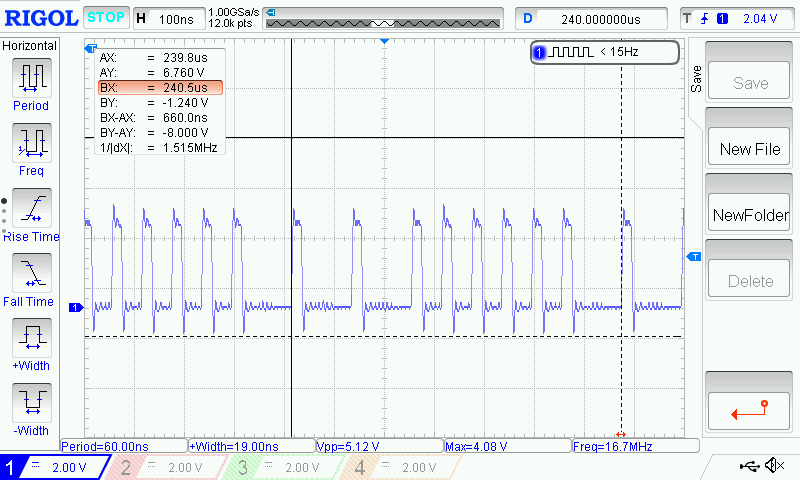
\includegraphics[scale=0.5]{instr_clk_impl} }}%
    \qquad
    \subfloat[Xilinx iSim simulation view of the \textit{q\_debug\_instr\_clk} signal.]{{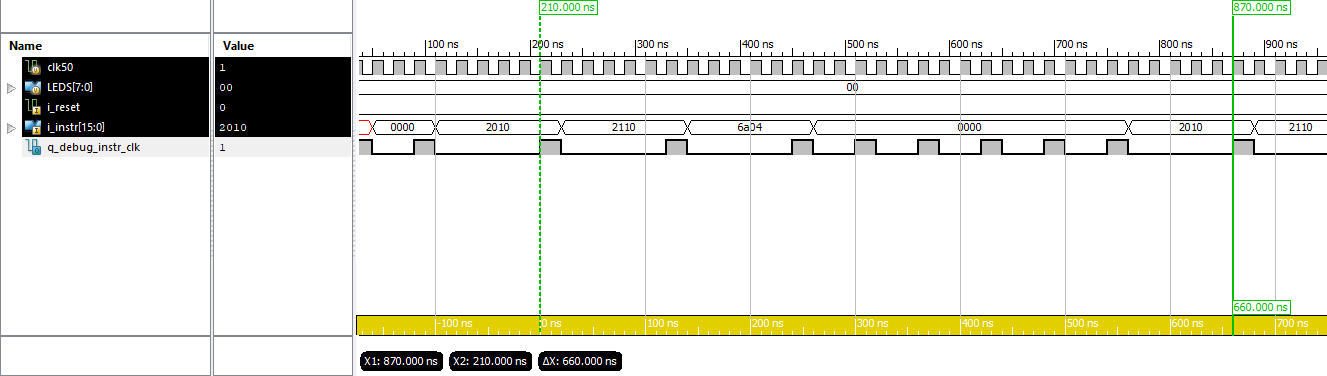
\includegraphics[scale=0.5]{instr_clk_sim} }}%
    \caption[]{Initial real-hardware implementation on the MiniSpartan6+ (XC6SLX9-3FTG256) development board showing timing of the \textit{q\_debug\_instr\_clk} signal. This signal is a 1 clock pulse indicating the start of an instruction cycle. In this example, instructions: MOVI \$10, \%Ra; MOVI \$10, \%Rb; and CMP \%Rc, \%Ra, \%Rb followed by 6 NOP instructions, are used.\newline\newline
    We can see that both implementations have a matching 660ns delay between instruction cycles for the same instructions, indicating that the real-hardware FPGA implementation is working correctly.}
    \label{fig:h5_impl}
\end{figure}

\newpage
\subsubsection*{Highlight 7}\label{inc:compiler_output}
Compiler input file contents:
\begin{minted}
[
linenos
]
{python}
def foo() {
    10 + 1;
}

def main() {
    32;
    foo();
}
\end{minted}

Compiler output machine code disassembly (pre-optimisation, post assembling):
\begin{minted}
[
linenos
]
{text}
0x00    ADDI    $-1,    Sp      4fff    Function/sf entry
0x01    SW      Bp,     +0(Sp)  16e0    (null)
0x02    MOV     Bp,     Sp      1ee0    main
0x03    MOVI    $20,    Ax      2020    NUMBER
0x04    MOVI    $9,     Cx      2209    Create return address
0x05    ADDI    $-1,    Sp      4fff    (null)
0x06    SW      Cx,     +0(Sp)  12e0    PUSH
0x07    MOVI    $d,     Cx      220d    call
0x08    JMP     Cx              6200    JMP
0x09    MOV     Sp,     Bp      1fc0    Function/sf exit
0x0A    LW      Bp,     +0(Sp)  0ee0    POP
0x0B    ADDI    $+1,    Sp      4f01    (null)
0x0C    HALT                    9000    MAIN HALT
------------------------------------
0x0D    ADDI    $-1,    Sp      4fff    Function/sf entry
0x0E    SW      Bp,     +0(Sp)  16e0    (null)
0x0F    MOV     Bp,     Sp      1ee0    foo
0x10    MOVI    $a,     Ax      200a    NUMBER
0x11    ADDI    $-1,    Sp      4fff    (null)
0x12    SW      Ax,     +0(Sp)  10e0    PUSH
0x13    MOVI    $1,     Ax      2001    NUMBER
0x14    LW      Cx,     +0(Sp)  0ae0    POP
0x15    ADDI    $+1,    Sp      4f01    (null)
0x16    ADD     Ax,     Cx      4040    BIN ADD
0x17    MOV     Sp,     Bp      1fc0    Function/sf exit
0x18    LW      Bp,     +0(Sp)  0ee0    POP
0x19    ADDI    $+1,    Sp      4f01    (null)
0x1A    LW      Cx,     +0(Sp)  0ae0    POP
0x1B    ADDI    $+1,    Sp      4f01    (null)
0x1C    JMP     Cx              6200    FUNC RETURN to CALL
\end{minted}


\newpage
\begin{landscape}
\subsection{Project Management Kanban Board}
\begin{figure}[H]
\centering
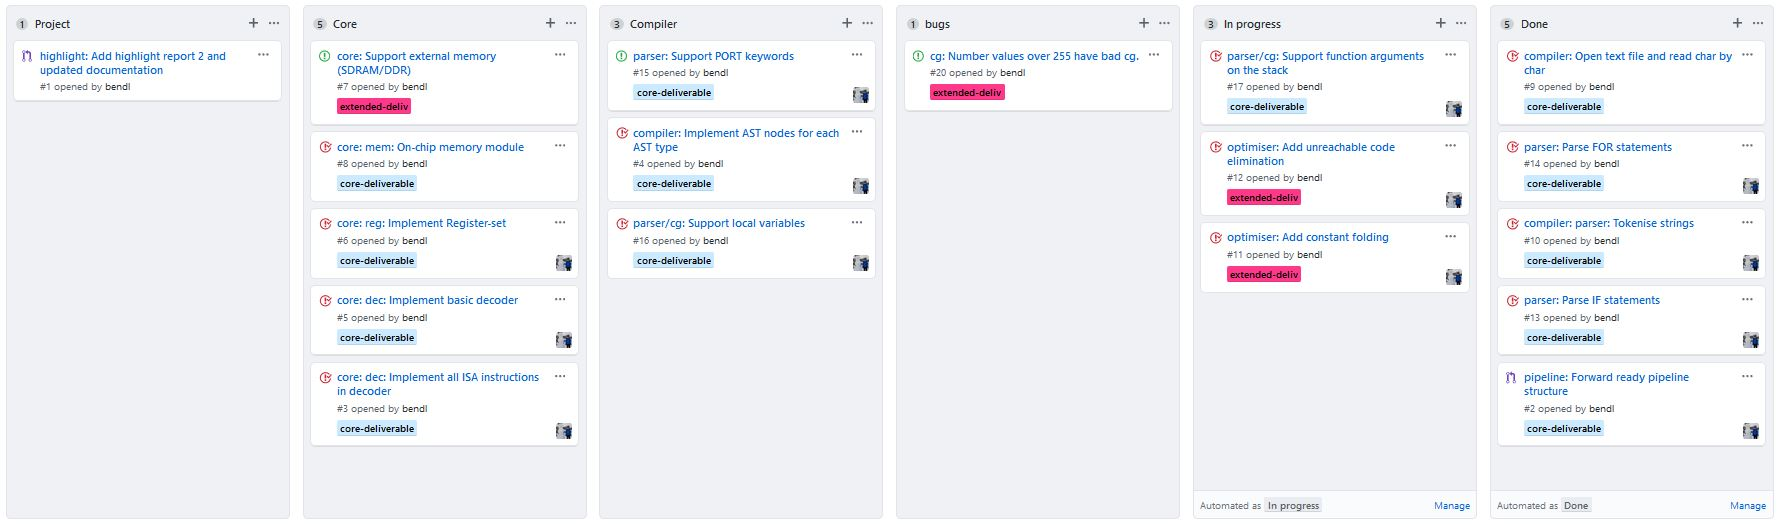
\includegraphics[scale=0.55]{kanban2}
\caption{Project Kanban board showing the status of different tasks of the project, processor core, and compiler. In addition, their requirements are shown (\textit{core-deliverable} and \textit{extended-deliv}), their task status (open, closed, merged), and who is assigned to each task. This kanban board can viewed at: \url{https://github.com/bendl/prco304/projects/1}.}
\label{kanban}
\end{figure}
\end{landscape}


\newpage
\section{Appendix C. Other Documents}
\subsection{Existing Embedded Processor and Compiler Research}
\label{current_impl}
There exists many commercial and open-source embedded processors, each providing different features and specialities such as digital signal processing, analogue components, instruction set architectures, and interfaces.

Popular embedded processors include:
\begin{itemize}
\item{\textit{Xilinx MicroBlaze \cite{microblaze}.} MicroBlaze features a 32-bit big-endian RISC architecture targeting FPGA devices. 

The processor's instruction set contains over 100 instructions, covering traditional RISC operations such as arithmetic (ADD), comparison (CMP), floating point operations (FADD), bitwise (XOR), memory operations (LW, SW). Interestingly, the processor allows full control of the program counter, and provides multiple instructions for controlling it.

MicroBlaze features 32 32-bit general purpose registers similar to other RISC architectures (ARMv8-A) with 32 32-bit general purpose registers). The high register count allows for storing of more values over the lifetime of programs, increasing performance by reducing timely memory operations.

The processor can included in FPGA designs using a graphical configuration tool, the MicroBlaze Configuration Wizard. This allows the designer to customise the features and implementation of the processor in their design. Designers can choose to integrate: commercial interface features, such as PCI Express interfaces; additional functionality, such as memory management units and floating point units; and performance features, such as instruction caching, and hardware multipliers/dividers.

\begin{figure}[H]
\centering
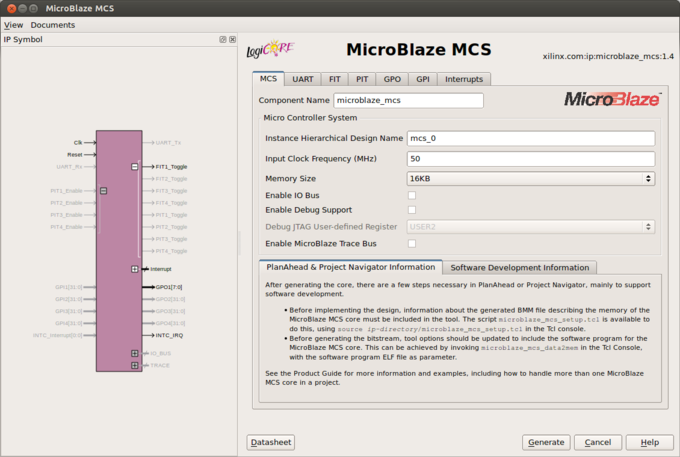
\includegraphics[scale=0.5]{mcw2}
\caption{The MicroBlaze Configuration Wizard, showing options for clock frequency, memory sizes, UART, GPIO, interrupts, and more. Source: \url{https://embeddedmicro.com/blogs/tutorials/embedded-processors}}
\end{figure}
}



\item{\textit{ARM Cortex-A9 MPCore} \cite{cortexa9}. The Cortex-A9 implements ARM's 32-bit Thumb-2 RISC instruction set. This architecture supports 15 32-bit registers, half of what MicroBlaze supports.

In addition to FPGA-based implementation, the Cortex-A9 is also designed for silicon based SoC designs. The processor is implemented in many commercial SoC products such as Broadcom's BCM11311, STMicroelectronics' SPEAr1310, and Apple's A5 mobile chip. }

\item{\textit{Xilinx PicoBlaze \cite{picoblaze}.} PicoBlaze is an  8-bit RISC embedded microcontroller, designed by Ken Chapman \cite{merchant2009platform}, originally named KCPSM ("Ken Chapman's Programmable State Machine") \cite{kamat2009unleash}.

An important characteristic of the PicoBlaze embedded processor is that it only requires a minimum of 26 FPGA slices, meaning that implementation on a Spartan-6 (XC6SLX9) FPGA that has 1430 slices, where each consists of 4-LUTs and 8 Flip Flops  \cite{spartan6}, results in only 1.8\% of the resources being used, allowing for more complex logic to be bundled alongside the processor. This low resource requirement is a key characteristic that designers use when considering embedded processors and will be considered in the design of the new embedded processor.
}
\end{itemize}

\subsection{Current Compiler Toolchains}
To run functional and complex programs on the processor, a high-level code compiler will be required. This compiler must be able to take a high-level grammar as input and output an executable that the new processor can run. Only open-source compilers will be considered due to having better documentation and source code, which reduces risk in the project. The source code will need to be open and modifiable as this project requires a backend to be implemented.

\begin{itemize}
\item{\textit{LLVM} \cite{llvm}. LLVM is a set of reusable compiler technologies that allows developers to build frontends, backends, and optimisers, for different projects. LLVM uses a text-based intermediate representation (IR). This IR is relocatable, allowing front-ends of multiple input grammars to be compiled to it, and back-ends to accept it to generate implementation specific code. 

LLVM, while a large project and still actively developed and used by many programming languages, such as Clang, Haskell, and Swift, suffers from poor and outdated documentation. This will be a large risk factor if chosen for this project as additional time will be required for learning it.
}


\item{\textit{8cc} \cite{8ccgithub}. 8cc is a small, open-source, C compiler built by Rui Ueyama.

The compiler is the simplest of the above mentioned compilers as it was only developed in 40 days \cite{8cc}. Although not fully implementing a standards compliant language,  the compiler is still functional and has the ability to compile itself (self-hosting) which is a great achievement.

The compiler does not assemble an executable file, but rather outputs x86\_64 AT\&T syntax assembly language. This is then assembled by a third-party assembler such as GCC's \textit{as} tool.

The project's source code is "written to be as concise and easy-to-read as possible" \cite{8cc} and this is indeed true looking at the contents. Although little documentation is available, the code generation functions of importance to this project in \textit{gen.c}, can be easily modified to emit our new instruction set architecture machine code.

Utilising this compiler will allow this processor to run more complex and functional programs. The disadvantage lies in the complexity of the C programming language, in that it requires many code generation routines for different variations of each program. To even compile a simple addition function, I will first need to implement many unused code generation routines such as datatype conversions, variable allocations, and more. In addition, some of these routines may not be implementable on the new processor and will result in undefined behaviour. This is a large risk to the project as an unknown amount of time will need to be allocated to create a backend for the compiler.
}
\end{itemize}

\begin{table}[H]
\def\arraystretch{1.5}
\begin{tabularx}{\textwidth}{|l|l|l|l|p{2cm}|X|}
\hline 
Processor & Architecture & Bits & Registers & Branching & Other \\ 
\specialrule{2pt}{-2pt}{0pt}

MicroBlaze & RISC & 32 & 32 & Branch on Condition, Condition & Interrupt Vector \\ 
\hline
ARMv8 & RISC & 32 & 31 & Condition & Interrupt Vector \\ 
\hline 
PicoBlaze & RISC & 8 & 16 & Condition & Internal 64-byte scratch memory;\newline 1KB Instruction on-chip storage;\newline Interrupts; 0.5 IPC \\ 
\hline 
\end{tabularx}
\caption{Comparison of existing embedded processor architectures.}
\label{sect:existing_isa_cmp}
\end{table} 

\newpage
\subsection{Compiler Functional Requirements}
\label{sect:compiler_func_req}
\begin{figure}[H]
\begin{center}
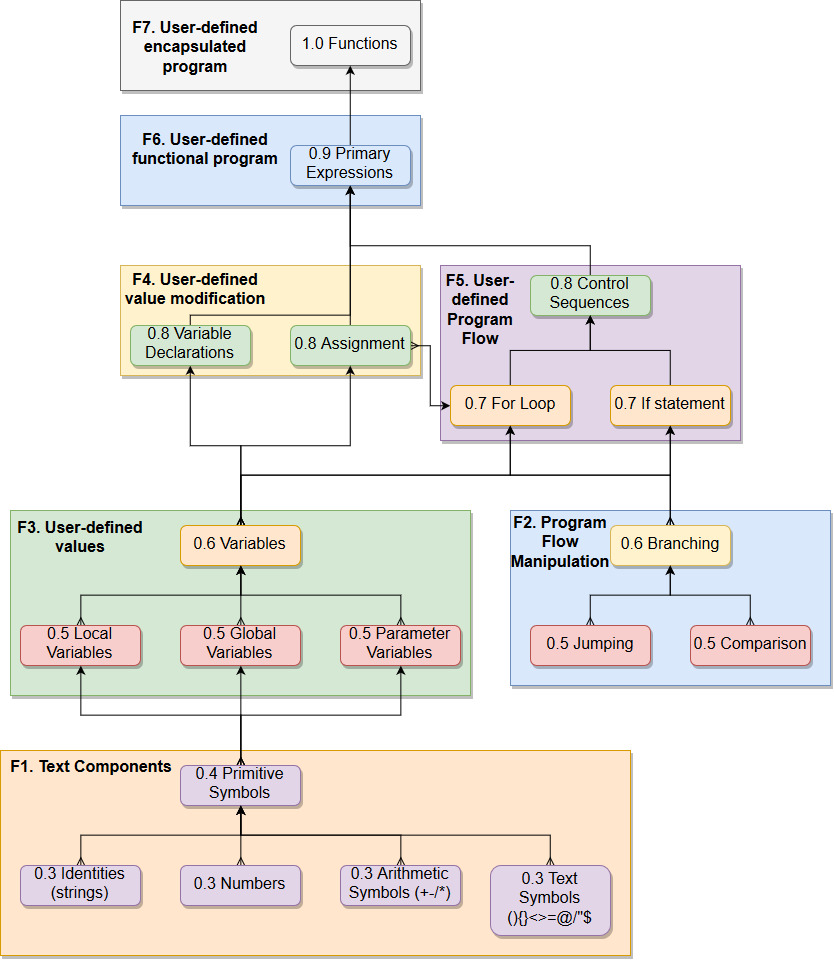
\includegraphics[scale=0.5]{compiler_dependencies}
\end{center}
\caption{\scname{} compiler Functional requirements and their technical implementation requirements. This diagram shows the technical implementation dependencies of each feature required by the compiler.}
\label{fig:compiler_dependencies}
\end{figure}

\scriptsize
Starting at \textit{F1}, we can see that the compiler needs to support strings, numbers, and arithmetic and text symbols, in order to support more complex features, such as user-defined variables. With \textit{F5}, to support user-defined program flow, such as \textit{if} and \textit{for} loops, we need the compiler to first support primitive jumping and comparison features. The higher up the functional requirement list, the more technical implemented features need to be present in order to support the feature. The highest functional requirement, \textit{F7}, will allow users to encapsulate programs into multiple functions, but in order to support this, the compiler must first implement program code, such as \textit{if(x) then y else z}.\\\\Structuring technical requirements in this format allows for better visualisation of their technical dependencies which leads to better informed time allocations for each task.
\normalsize

\subsection{Compiler Sequence Diagram}
\label{sect:compiler_seq_uml}
\begin{figure}[H]
\begin{center}
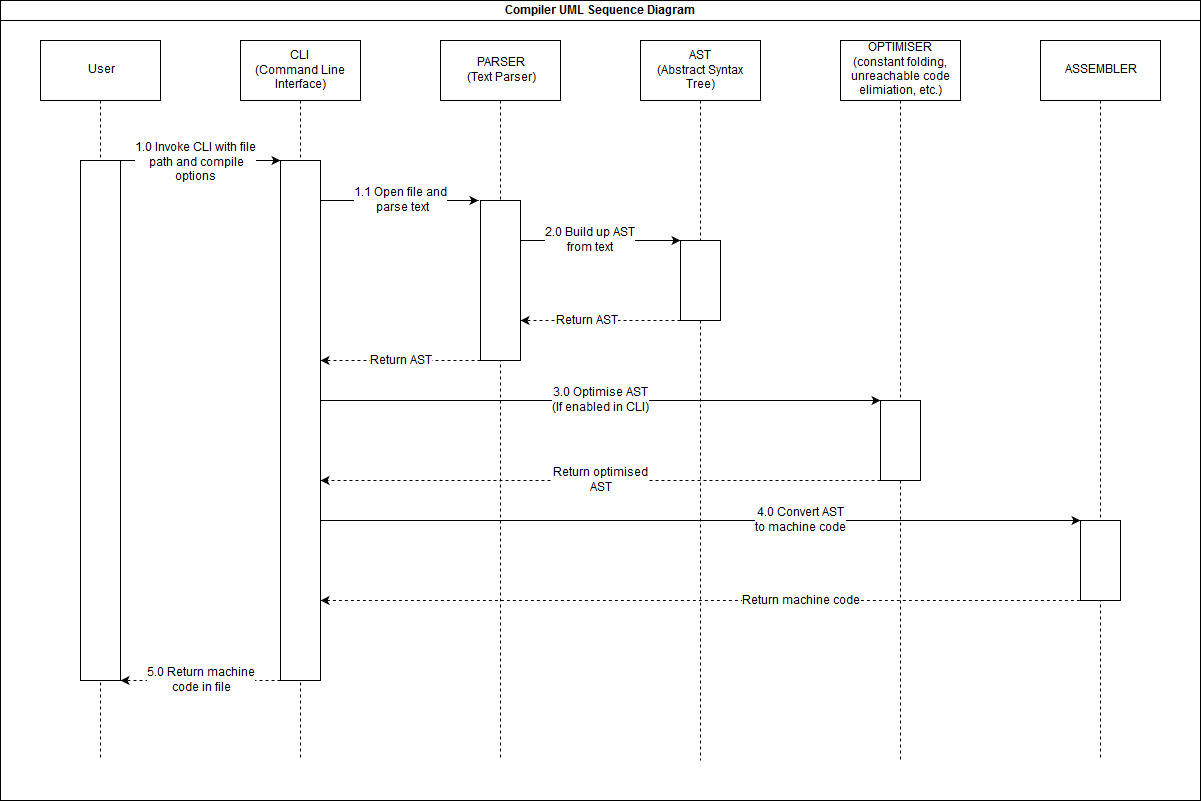
\includegraphics[scale=0.4]{fig_compiler_uml_seq}
\end{center}
\caption{UML sequence diagram for the \scname{} compiler. This diagram shows the compiler's program flow. The CLI is the only component the user is required to interact with. The user passes the input file to the CLI which in-turn invokes the compiler to parse and generate output machine code.}
\label{fig:hld}
\end{figure}

\newpage
\subsection{ISE XC6SLX9 Implementation Report}
\label{ise_report}
\begin{figure}[H]
    \begin{minipage}{0.5\textwidth}
        \centering
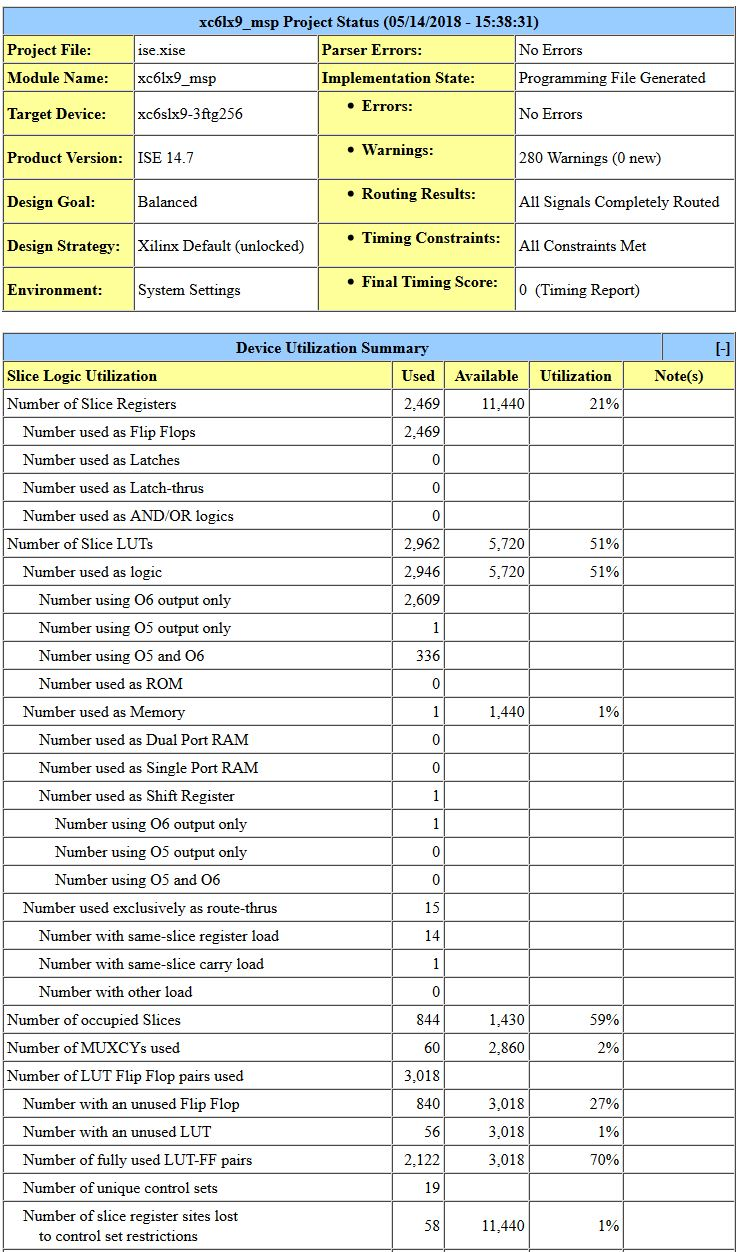
\includegraphics[scale=0.43]{ise1}
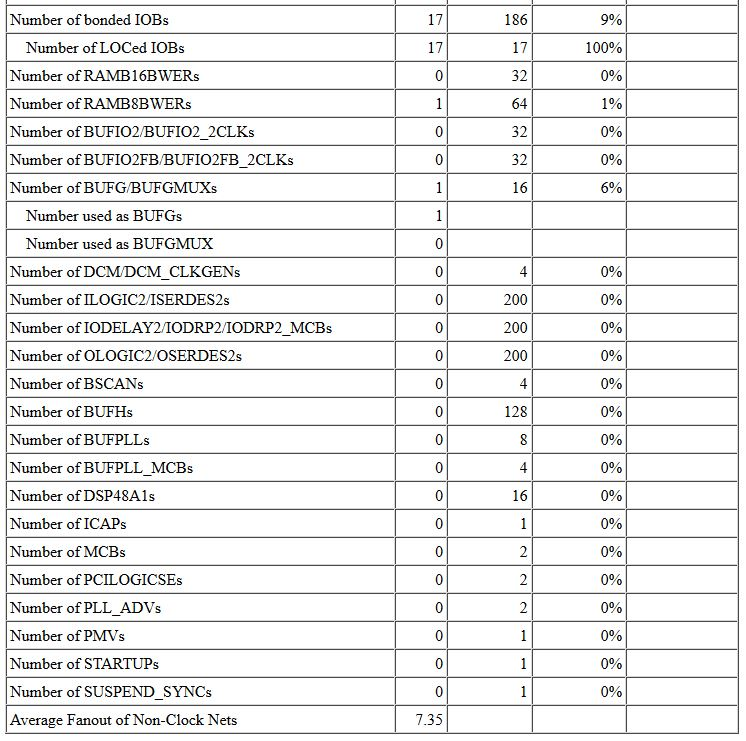
\includegraphics[scale=0.43]{ise2}
    \end{minipage}
    \begin{minipage}{0.01\textwidth}\hfill\end{minipage}
    \begin{minipage}{0.5\textwidth}
        \centering
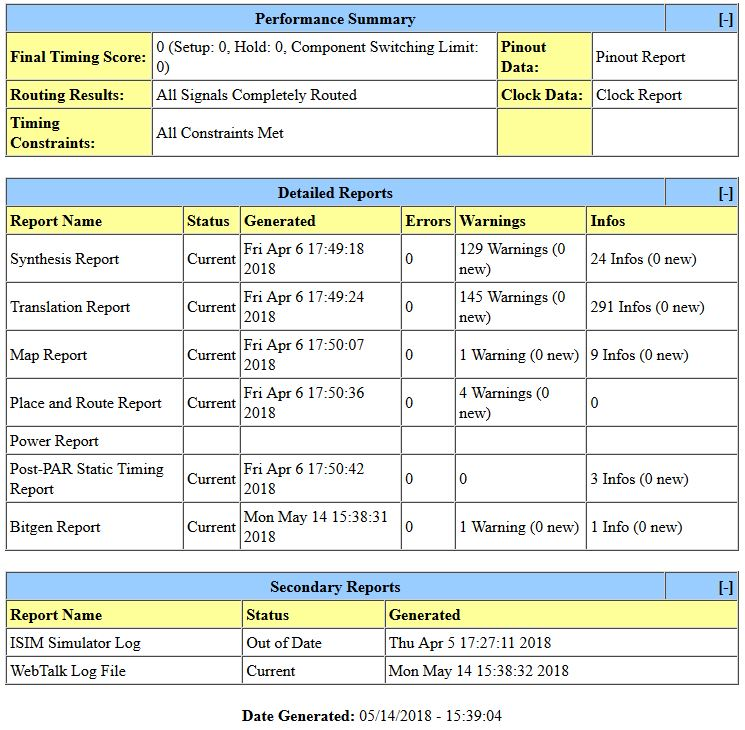
\includegraphics[scale=0.45]{ise3}\\
    \end{minipage}
    \caption{ISE implementation report for the \scname{} processor on the XC6SLX9 FPGA device.}
    \label{fig:}
\end{figure}


%TC:endignore
\end{document}
